\documentclass[
11pt, % The default document font size, options: 10pt, 11pt, 12pt
%oneside, % Two side (alternating margins) for binding by default, uncomment to switch to one side
italian, 
singlespacing, % Single line spacing, alternatives: onehalfspacing or doublespacing
%draft, % Uncomment to enable draft mode (no pictures, no links, overfull hboxes indicated)
%nolistspacing, % If the document is onehalfspacing or doublespacing, uncomment this to set spacing in lists to single
%liststotoc, % Uncomment to add the list of figures/tables/etc to the table of contents
%toctotoc, % Uncomment to add the main table of contents to the table of contents
%parskip, % Uncomment to add space between paragraphs
%nohyperref, % Uncomment to not load the hyperref package
headsepline, % Uncomment to get a line under the header
%chapterinoneline, % Uncomment to place the chapter title next to the number on one line
%consistentlayout, % Uncomment to change the layout of the declaration, abstract and acknowledgements pages to match the default layout
]{MastersDoctoralThesis} % The class file specifying the document structure

\usepackage[utf8]{inputenc} % Required for inputting international characters
\usepackage[T1]{fontenc} % Output font encoding for international characters
\usepackage{amsmath}
\usepackage{verbatim}
\usepackage{amsfonts}
\usepackage{siunitx}
\usepackage{subfloat}
\usepackage{changepage}
\usepackage{float}
\usepackage{subfig}
\usepackage{textcomp}
\usepackage{enumitem}
\usepackage{hyperref}
\usepackage{lmodern} % Use the Palatino font by default
\usepackage{eso-pic}
\usepackage{parskip}
\usepackage{setspace}
\usepackage[nottoc]{tocbibind}
\usepackage{diagbox}
\usepackage{nicefrac}
\usepackage[autostyle=true]{csquotes} % Required to generate language-dependent quotes in the bibliography
\usepackage{amsthm}
\usepackage[backend=bibtex,style=ieee,natbib=true]{biblatex} % Use the bibtex backend with the authoryear citation style (which resembles APA)à
\usepackage{footmisc}

\theoremstyle{plain} 
\newtheorem{thm}{Theorem}[section] 
\newtheorem{cor}[thm]{Corollary} 
\newtheorem{lem}[thm]{Lemma} 
\newtheorem{prop}[thm]{Proposition} 

\theoremstyle{definition} 
\newtheorem{defn}{Definition}[chapter] 

\theoremstyle{remark} 
\newtheorem{obs}{Observation} 

\newcommand\alcentropagina[1]{\AddToShipoutPicture{%
		\AtPageCenter{\makebox(50,0){\includegraphics[width=1.2\textwidth]{#1}}}}}

%	MARGIN SETTINGS

\geometry{
	paper=a4paper, % Change to letterpaper for US letter
	inner=3.8cm, % Inner margin 
	outer=3.8cm, % Outer margin
	bindingoffset=.5cm, % Binding offset
	top=1.5cm, % Top margin
	bottom=1.5cm, % Bottom margin
	%showframe, % Uncomment to show how the type block is set on the page
}

%INFO

\supervisor{Fulvio \textsc{Corno}} % Your supervisor's name, this is used in the title page, print it elsewhere with \supname
\degree{Ingegneria Gestionale L8} % Your degree name, this is used in the title page and abstract, print it elsewhere with \degreename
\author{Mario Francesco Pio  \textsc{Lapadula}} % Your name, this is used in the title page and abstract, print it elsewhere with \authorname
\keywords{} % Keywords for your thesis, this is not currently used anywhere in the template, print it elsewhere with \keywordnames
\university{Politecnico di Torino} % Your university's name and URL, this is used in the title page and abstract, print it elsewhere with \univname
\thesistitle{Applicazione gestionale per la simulazione di una stagione di F1 2024} % Your thesis title, this is used in the title and abstract,

\AtBeginDocument{
\hypersetup{pdftitle=\ttitle} % Set the PDF's title to your title
\hypersetup{pdfauthor=\authorname} % Set the PDF's author to your name
\hypersetup{pdfkeywords=\keywordnames} % Set the PDF's keywords to your keywords
}

\begin{document}

%----------------------------------- FRONTESPIZIO GRANDE ----------------------
\newgeometry{
	paper=a4paper, % Change to letterpaper for US letter
	inner=3cm, % Inner margin
	outer=2.5cm, % Outer margin
	bindingoffset=.5cm, % Binding offset
	top=3.5cm, % Top margin
	bottom=1.5cm, % Bottom margin
}

%%%%%%%%%%%%%%%%%% PRIMA PAGINA %%%%%%%%%%%%%%%%%%

% Use roman page numbering style (i, ii, iii, iv...) for the pre-content pages

\pagestyle{plain} % Default to the plain heading style until the thesis style is called for the body content
\begin{titlepage}
	\begin{center}
		
		
\includegraphics[scale=0.27]{Figures/logo.jpg} % University/department logo - uncomment to place it
            
		%\vspace*{.06\textheight}  
		{\color{black}{\scshape\LARGE \univname \par}\vspace{1.2cm}} % University name
		
		\textsc{\Large Laurea Triennale in
			\degreename}\\[0.5cm] % Thesis type
		
		\HRule \\[2cm] % Horizontal line
		{\huge \bfseries \ttitle\par}\vspace{1cm} % Thesis title
		
		\begin{minipage}[t]{0.4\textwidth}
			\begin{flushleft} \large
				\emph{Candidato}\\
				\href{}{\authorname} % Author name - remove the \href bracket to remove the link
			\end{flushleft}
		\end{minipage}
		\begin{minipage}[t]{0.4\textwidth}
			\begin{flushright} \large
				\emph{Relatore} \\
				\href{}{\supname} \\ % Supervisor name - remove the \href bracket to remove the link  
				\phantom{null}\newline 
			\end{flushright}
		\end{minipage}\\[2cm]
		
		\vfill
  
		\vfill
		\HRule \\[1cm] % Horizontal line
		{\large ANNO ACCADEMICO 2023/2024 }\\[4cm] 
		
		\vfill
	\end{center}


\cleardoublepage

%----------------------------------------------------------------------------------------
%	TITLE PAGE
%----------------------------------------------------------------------------------------


	\begin{center}
 
		\vspace{21cm}
		%
		% Autore
		\makeatletter
		\large\textrm{\authorname}
		\makeatother
		\vspace{8.85cm}
		%
		% Titolo
		\begin{center}
			\makeatletter
			\singlespacing\Huge\textsc{\ttitle}
			\makeatother
		\end{center}%
		\vspace{0.4cm}
		%
		% Tipo di Tesi
		\makeatletter
		\large\textit{Tesi di Laurea Triennale}
		\makeatother
		\vfill
		%
		\large POLITECNICO DI TORINO\\
		\vspace{1cm}
		%
		% Data Esame di Laurea
		\makeatletter
		\large\textrm{Luglio 2024} % Add month and year of your graduation
		\makeatother
	\end{center}
\end{titlepage}

\restoregeometry

\pagestyle{plain} % Default to the plain heading style until the thesis style is called for the body content

%----------------------------------------------------------------------------------------
%	LIST OF CONTENTS/FIGURES/TABLES PAGES
%----------------------------------------------------------------------------------------
\frontmatter % Use roman page numbering style (i, ii, iii, iv...) for the pre-content pages

\tableofcontents % Prints the main table of contents

\listoffigures % Prints the list of figures

%	THESIS CONTENT - CHAPTERS
%----------------------------------------------------------------------------------------

\mainmatter % Begin numeric (1,2,3...) page numbering

\pagestyle{thesis} % Return the page headers back to the "thesis" style

% Include the chapters of the thesis as separate files from the Chapters folder

\chapter{Proposta di progetto}

\label{Capitolo1}

\section{Titolo della proposta}
Simulazione di una stagione di F1 gestendo lo sviluppo tecnico di una scuderia

\section{Descrizione del problema proposto}
L’applicazione permette di indossare i panni di una scuderia di F1 e simulare una stagione avendo la possibilità di investire una somma di denaro limitata in quattro diversi reparti tecnici. È inoltre possibile cambiare i piloti della propria squadra prima dell’inizio della stagione. Tramite un numero elevato di simulazioni si potrà capire qual è la miglior coppia di piloti e il miglior piano di investimenti per massimizzare il risultato del team.

\section{Descrizione della rilevanza gestionale del problema}
In F1 è in vigore un regolamento che impone una somma di denaro massima per lo sviluppo della vettura per garantire parità di condizioni di partenza tra i vari team, dunque la scelta e il bilanciamento dei vari investimenti sono fondamentali.
La sfida gestionale consiste nell’ottimizzazione di una strategia di investimento nei vari settori tecnici, verificando quanto ogni diversa combinazione di asset possa apportare cambiamenti sul rendimento finale.
È importante valutare l’investimento in relazione alle caratteristiche del team scelto nella simulazione, in quanto potrebbe essere poco efficace andare ad investire tanto su un reparto in cui si è già abbastanza competitivi.
È particolarmente significativa anche la scelta dei due piloti per massimizzare il rendimento della scuderia.

\section{Descrizione dei data-set per la valutazione}
L’applicazione fa uso di diversi dataset:

\begin{itemize}
    \item statistiche qualitative dei piloti rilasciate dal videogioco F1 Manager 2023\footnote{che detiene la licenza ufficiale della F1};
    \item statistiche tecniche sui circuiti di gara dal sito \url{https://tracks.f1setup.it/};
    \item statistiche tecniche delle scuderie estratte dal videogioco F1 2023\footnotemark[1] prodotto da Codemaster e EA;
    \item statistiche qualitative sullo staff tecnico di ogni team estratte dal videogioco F1 Manager 2023\footnotemark[1];
    \item tempo di percorrenza della pit-lane per ogni circuito, rilasciato da IGP Manager;
    \item probabilità di pioggia calcolato rispetto alla frequenza di pioggia in determinato circuito \footnote{calcolato tenendo in considerazione le ultime 15 gare disputate sul determinato circuito};
    \item indice di probabilità di un sorpasso calcolato per ogni circuito tramite la media dei sorpassi avvenuti nelle gare disputate dal 2010 al 2024 (dati estratti dal sito \url{https://www.statsf1.com/it/default.aspx});
    \item tempo di percorrenza del giro basato sul giro più veloce effettuato nell’ultima gara disputata nello specifico circuito in esame (dati su gare avvenute prima della stagione 2024).
\end{itemize}

\section{Descrizione preliminare degli algoritmi coinvolti}
Il principale algoritmo coinvolto è una simulazione a eventi discreti.
L’intera stagione è divisa in eventi chiamati ‘Sessione’ che a loro volta saranno divisi in ‘Qualifica’ e ‘Gara’. C’è una ‘Sessione’ per ogni appuntamento nel calendario della stagione.
All’inizio di ogni ‘Sessione’ di gara vengono calcolati gli indici di prestazione delle vetture dei vari team in base ai dati tecnici disponibili nel database e correlati alle caratteristiche della pista che ospiterà il weekend di gara.

Esempio: sul tracciato di Montecarlo, che presenta un rapporto bassissimo rettilinei/curve e curve strette, sono più competitive le vetture che presentano un buon livello di aerodinamica e/o telaio, mentre non pesa granché il dato sulla qualità del reparto motoristico.

Dopodiché si calcolano anche le prestazioni dei piloti in base alla pista.

Esempio: un pilota con alti valori di gestione gomma su una pista con un alto consumo gomme ha un’ottima prestazione.

Dopo aver calibrato le prestazioni di vetture e piloti in base al circuito si procede con la simulazione delle qualifiche che stabilisce la griglia di partenza per la gara. Nella simulazione della qualifica vengono prese in considerazione le prestazioni aggiornate dei team e alcune caratteristiche dei piloti legate alla velocità sul giro, combinati anche con fattori randomici.

Finita la simulazione delle qualifiche, inizia la simulazione della gara. La prima fase di gara è la partenza: in questo momento c’è un’alta possibilità per un pilota di compiere e/o subire un sorpasso. Dopo la partenza la gara procede in maniera lineare: in ogni giro i piloti segnano un tempo in base alle proprie statistiche combinate con fattori randomici. Se il distacco tra due piloti è inferiore a 1 secondo, si simula il tentativo di sorpasso. Durante la gara possono verificarsi eventi particolari, come incidenti, problemi tecnici, problemi al pit stop e pioggia. La probabilità di questi eventi è legata al tracciato che ospita la gara e a caratteristiche tecniche delle scuderie (es. affidabilità e qualità della pit crew), oltre che a variabili aleatorie. Alla fine della gara si stila l’ordine di arrivo e si assegnano i punteggi.

Alla fine di ogni ‘Sessione’ si aggiornano le classifiche. Questo iter prosegue fino alla fine della stagione di gara in corso.
A questo punto viene stilata la classifica finale per i piloti e per i costruttori.

\section{Descrizione preliminare delle funzionalità previste per l’applicazione software}
L’utente potrà scegliere la scuderia da gestire da un menu a tendina e potrà inserire l’importo da investire in ognuno dei quattro reparti tecnici in campi di testo dedicati. L’utente dovrà rimanere entro la somma massima di 140 milioni di dollari, imposta dal nuovo regolamento di F1. Se la somma non verrà rispettata, l’avvio della simulazione sarà impedito.

Tramite due ulteriori menu a tendina è possibile scegliere i due piloti che gareggeranno nella scuderia scelta. Il menu a tendina è popolato con tutti i piloti presenti attualmente in F1 e sarà inizializzato con i due piloti ingaggiati nel 2024 dal team scelto.
Una volta completato l’inserimento dei dati è possibile avviare la simulazione tramite un pulsante dedicato.

Completata la simulazione verranno visualizzati i risultati complessivi della scuderia e dei piloti della stessa affiancati da un riepilogo sugli investimenti effettuati. È possibile svolgere un numero illimitato di simulazioni, i cui risultati verranno mostrati in una tabella scorrevole tramite una seconda interfaccia grafica. La tabella sarà utile per confrontare i vari investimenti e trovare quello più proficuo per la scuderia scelta.

Nel caso del mancato inserimento dei dati o della presenza di errori compilativi delle caselle di testo, la simulazione non verrà avviata.
L’utente può liberare le caselle di testo della schermata simulativa con un pulsante ‘Cancella’ e azzerare i dati contenuti nella tabella con un pulsante ‘Azzera’.


\counterwithin{figure}{section}

\chapter{Descrizione dettagliata del problema affrontato}

\label{Capitolo 2}

Il campionato di F1 è il campionato di spicco nel mondo del motorsport: i 20 piloti più abili al mondo gareggiano sulle vetture da corsa più performanti per vincere il campionato mondiale. Questo palcoscenico offre, più che una sfida tra le abilità dei piloti in pista, una sfida ingegneristica e strategica tra le scuderie. In F1, la maggior parte delle volte, non vince il miglior pilota in pista ma quello che guida la vettura più veloce e più affidabile.
Per questo motivo il lavoro dietro le quinte di una stagione di Formula 1 è durissimo, volto continuamente ad un’estrema innovazione tecnica di concetti aerodinamici, motoristici e di efficienza. 
Ma dal 2021, al fine di rendere la competizione più equa, è stata introdotta una regola che impone un tetto massimo di spese per gli investimenti tecnici per migliorare la vettura. Fino ad allora spesso trionfava chi investiva più fondi nella ricerca e nello sviluppo della vettura, ma dall’emissione del nuovo regolamento la sfida tecnica si è fatta più avvincente.
Ciò ha reso la sfida ingegneristica e gestionale molto intensa, con i vari team che si vedono costretti a scegliere in quali aree di ricerca investire maggiormente il denaro. 
L’obiettivo dell’applicazione è quello di individuare il più vantaggioso asset di investimenti per massimizzare il rendimento della propria squadra e quindi aumentare le percentuali di successo nel campionato. 
Questo sarà possibile svolgendo un gran numero di simulazioni e verificando quanto ogni diversa combinazione di asset possa apportare cambiamenti sul rendimento finale.
Non vi è però un asset univoco per massimizzare le qualità di una vettura di F1: nella competizione sono presenti dieci tipologie di vetture con, di conseguenza, diverse qualità tecniche tra di loro.
Ogni vettura ha un’area tecnica in cui è più carente rispetto al livello medio delle scuderie ma non è detto che lo sviluppo di quell’area sia il più fruttuoso in termini di prestazioni.
L’applicazione permette quindi di svolgere un gran numero di simulazioni, scegliendo accuratamente dove e come investire i 140 milioni di dollari per poi visualizzare i risultati complessivi di fine stagione. Questi saranno visualizzati tramite le righe di una colonna che renderà semplice e immediato il confronto tra le simulazioni.
Non è da sottovalutare la scelta dei piloti: quando il livello delle vetture è vicino tra loro, è la scuderia con la miglior coppia di piloti ad avere la meglio. 
L’applicazione permette anche di scegliere la coppia di piloti per la scuderia selezionata: il giusto pilota permetterà alla scuderia di sovraperformare e raggiungere grandi risultati.
L’applicazione calibrerà il peso dell’investimento anche in base all’arretratezza tecnica del team scelto: è più facile e meno rischioso innovarsi ispirandosi a concetti già presenti in team rivali invece che ricercare nuove soluzioni.

\chapter{Descrizione del Dataset}

\label{Capitolo 3}

\section{Provenienza del Dataset}

Il dataset utilizzato per il funzionamento dell'applicazione è stato costruito manualmente per intero. Una grande quantità di dati è stata estratta dalle seguenti fonti:
\begin{itemize}
    \item F1 2023, videogioco prodotto da CodeMaster e EA con licenza ufficiale della F1;
    \item F1 Manager 2023, videogioco manageriale sviluppato da Frontier Developments con licenza ufficiale della F1;
    \item \url{https://tracks.f1setup.it/}, che contiene informazioni dei vari circuiti;
    \item \url{https://www.statsf1.com/it}, che contiene un database su ogni attività in pista avvenuta dal 1951 in Formula1;
    \item \url{https://steamcommunity.com/sharedfiles/filedetails/?id=3033340960}, una guida che contiene le informazioni tecniche dei circuiti.
\end{itemize}
L’intero database è disponibile in formato .txt da eseguire tramite un compilatore SQL. È reperibile nella cartella \texttt{LMFP/tree/master/src/main/java/it/polito/tdp/SimulazioneF1/db}.

\section{Contenuto del Dataset}

Il dataset contiene principalmente dati e informazioni su:
\begin{itemize}
    \item valutazioni qualitative dei piloti attualmente ingaggiati dai team;
    \item valutazioni qualitative delle vetture di ogni scuderia;
    \item informazioni identificative dei piloti, sui team e sui circuiti;
    \item dati tecnici per ogni circuito presente nel calendario 2024 del campionato di F1;
    \item numero di sorpassi effettuati per ogni circuito nelle edizioni disputate dal 2010 al 2023 (compresi).
\end{itemize}

\section{Struttura e Descrizione delle Tabelle}

\begin{figure}[htbp]
    \centering
    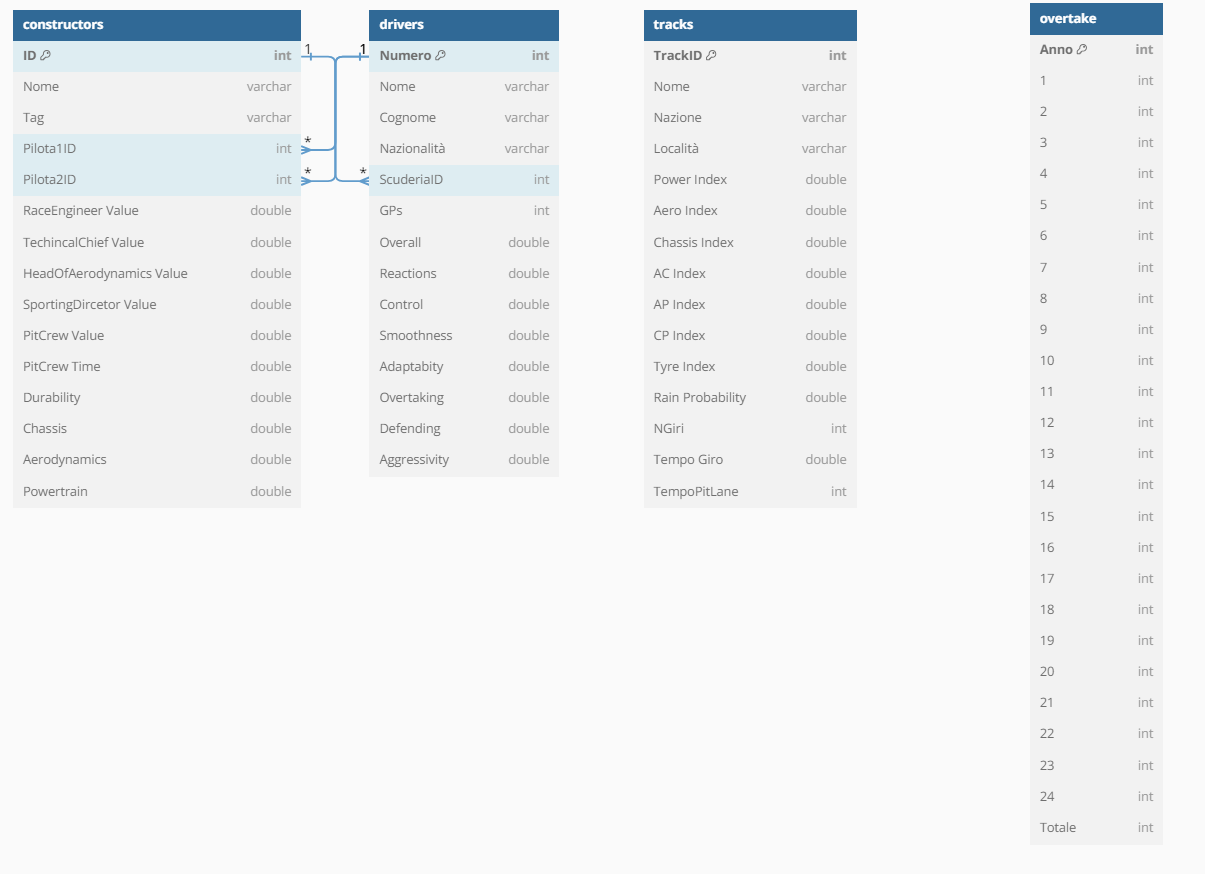
\includegraphics[width=\textwidth]{Figures/db.png}
    \caption{Diagramma di schema del database}
    \label{fig:database-schema}
\end{figure}

\subsection{Tabella Constructors}

La tabella \texttt{Constructors} contiene dati identificativi riguardanti i 10 team presenti attualmente in Formula 1 e dati qualitativi sulle rispettive vetture. \\
Descrizione delle colonne:
\begin{itemize}
    \item \texttt{ID}: numero che identifica univocamente il team;
    \item \texttt{Pilota1ID}: numero che descrive univocamente il pilota1 del team;
    \item \texttt{Pilota2ID}: numero che descrive univocamente il pilota2 del team;
    \item \texttt{Nome}: nome del team;
    \item \texttt{Tag}: abbreviazione di tre lettere del nome del team;
    \item \texttt{RaceEngineerValue}: indice qualitativo dell’ingegnere di gara del team;
    \item \texttt{TechnicalChiefValue}: indice qualitativo del capo dello sviluppo tecnico del team;
    \item \texttt{HeadOfAerodynamicsValue}: indice qualitativo del capo del settore aerodinamico del team;
    \item \texttt{PitCrewValue}: indice qualitativo sulla Pit Crew del team;
    \item \texttt{PitCrewTime}: tempo medio di pit stop effettuato dalla Pit Crew;
    \item \texttt{Durability}: indice qualitativo della resistenza dei componenti che costituiscono la vettura del team;
    \item \texttt{Chassis}: indice qualitativo del telaio della vettura del team;
    \item \texttt{Powertrain}: indice qualitativo del motore della vettura del team;
    \item \texttt{Aerodynamics}: indice qualitativo dell’aerodinamica della vettura del team;
\end{itemize}

\subsection{Tabella Drivers}

La tabella \texttt{Drivers} contiene dati identificativi sui 20 piloti che gareggiano attualmente in F1 e delle statistiche qualitative riguardo alle rispettive abilità di guida. \\
Descrizione delle colonne:
\begin{itemize}
    \item \texttt{Numero}: numero univoco che identifica la vettura che guida il pilota;
    \item \texttt{Nome}: nome del pilota;
    \item \texttt{Cognome}: cognome del pilota;
    \item \texttt{Nazionalità}: nazionalità del pilota;
    \item \texttt{ScuderiaID}: codice identificativo della scuderia del pilota;
    \item \texttt{GPs}: numero di GP disputati dal pilota prima dell’inizio della stagione 2024;
    \item \texttt{Overall}: indice qualitativo totale dell’abilità di guida del pilota;
    \item \texttt{Reactions}: indice sulla capacità di reazione ad imprevisti del pilota;
    \item \texttt{Control}: indice sul controllo in situazioni particolari della guida del pilota;
    \item \texttt{Smoothness}: indice sull’abilità di gestire le gomme del pilota;
    \item \texttt{Adaptability}: indice sull’abilità di adattamento del pilota;
    \item \texttt{Overtaking}: indice sull’abilità del sorpasso del pilota;
    \item \texttt{Defending}: indice sulla capacità di difesa del pilota;
    \item \texttt{Aggressivity}: indice sull’aggressività di guida del pilota;
\end{itemize}

\subsection{Tabella Tracks}

La tabella \texttt{Tracks} contiene dati identificativi del circuito, oltre agli indici che indicano quanto il circuito si presti ad una determinata qualità tecnica delle vetture (aerodinamica, telaio, motore). \\
Descrizione delle colonne:
\begin{itemize}
    \item \texttt{TrackID}: numero identificativo univoco del circuito;
    \item \texttt{Nome}: nome esteso del circuito;
    \item \texttt{Nazione}: nazione in cui è situato il circuito;
    \item \texttt{Località}: località in cui è situato il circuito;
    \item \texttt{Power Index}: indice sull’importanza del motore sulla prestazione nel circuito;
    \item \texttt{Aero Index}: indice sull’importanza dell’aerodinamica sulla prestazione nel circuito;
    \item \texttt{Chassis Index}: indice sull’importanza del telaio sulla prestazione nel circuito;
    \item \texttt{AC Index}: indice di correlazione sull’importanza aerodinamica - telaio sulla prestazione nel circuito;
    \item \texttt{AP Index}: indice di correlazione sull’importanza aerodinamica - motore sulla prestazione nel circuito;
    \item \texttt{CP Index}: indice di correlazione sull’importanza motore - telaio sulla prestazione nel circuito;
    \item \texttt{Tyre Index}: indice sul consumo gomma del circuito;
    \item \texttt{Rain Probability}: probabilità di pioggia sul circuito;
    \item \texttt{NGiri}: numero di giri della gara disputata sul circuito;
    \item \texttt{Tempo Giro}: tempo in secondi di percorrenza in condizioni ideali del circuito;
    \item \texttt{TempoPitLane}: tempo medio in secondi di percorrenza della Pit Lane del circuito durante un pit stop;
\end{itemize}

\subsection{Tabella Overtake}

La tabella \texttt{Overtake} contiene il numero di sorpassi effettuati in un circuito per ogni anno nelle gare disputate dal 2010 al 2023 (compresi). La tabella è stata creata con i codici identificativi dei circuiti come colonne per facilitare l’estrazione e l’analisi dei dati. È utilizzata solamente per calcolare un indice di probabilità di sorpasso, attributo di un’istanza Circuito.



%\counterwithin{figure}{section}

\chapter{Funzionamento dell'applicazione}

\section{Descrizione dei controller}
L’applicazione dispone di due controller:
\begin{itemize}
    \item \textbf{FXMLController}, gestisce la parte simulativa permettendo di impostare e avviare la simulazione;
    \item \textbf{RisultatiController2}, permette la visualizzazione in forma tabulare delle varie simulazioni effettuate.
\end{itemize}
\newpage
\section{Impostazione dei parametri di simulazione}
All’avvio della simulazione, verrà visualizzata la prima View \textit{Scene.fxml} (Figura \ref{fig:scene_fxml}), tramite la quale è possibile impostare i vari parametri simulativi inserendoli in caselle di testo e scegliendo tra opzioni disponibili nelle \textit{ComboBox}.

\begin{figure}[h!]
    \centering
    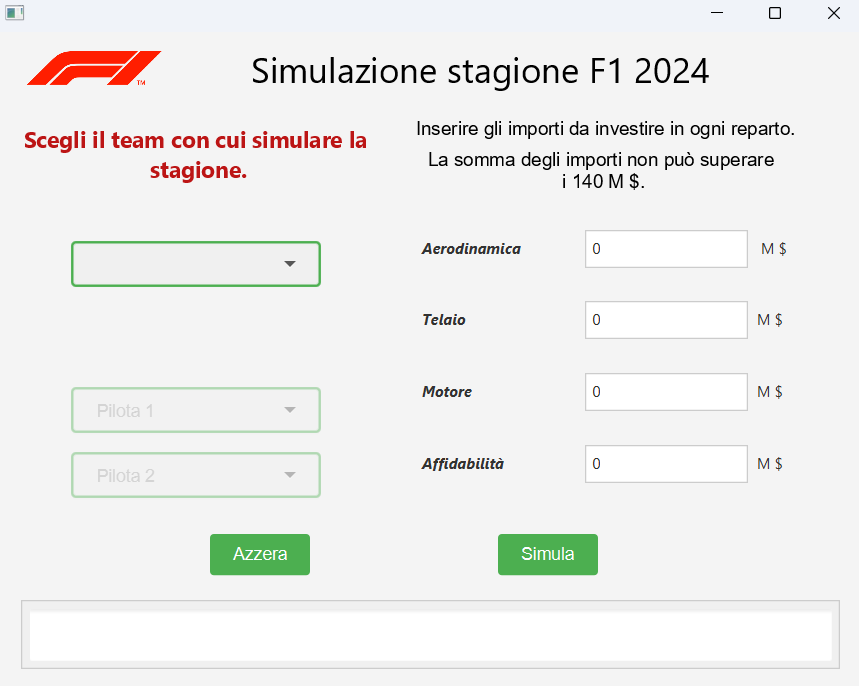
\includegraphics[width=0.8\linewidth]{Figures/schermata1.png}
    \caption{View Scene.fxml}
    \label{fig:scene_fxml}
\end{figure}

I parametri che possono essere impostati sono:
\begin{itemize}
    \item \textbf{Scuderia} in cui poter investire, tramite \textit{ComboBox};
    \item La coppia di \textbf{piloti} che gareggeranno per la scuderia scelta, tramite \textit{ComboBox};
    \item Il valore dell’\textbf{investimento} nei vari settori (\textit{Aerodinamica, Telaio, Motore, Affidabilità}), tramite caselle di testo.
\end{itemize}

L’unica limitazione riguarda la somma dei valori dell’investimento che non può superare i 140M \$. Se questa regola non è rispettata o se l’inserimento dei dati non è svolto correttamente, l’applicazione non permetterà di avviare la simulazione segnalando l’errore. Sono presenti due pulsanti, ‘\textit{Azzera}’ e ‘\textit{Simula}’, grazie ai quali è possibile ripristinare ai valori standard i vari campi editabili o iniziare la simulazione.
\newpage
\section{Visualizzazione dei risultati}
Dopo l’avvio della simulazione, si verrà trasferiti ad un’altra View \textit{Risultati2.fxml} (Figura \ref{fig:risultati_fxml}).

\begin{figure}[h!]
    \centering
    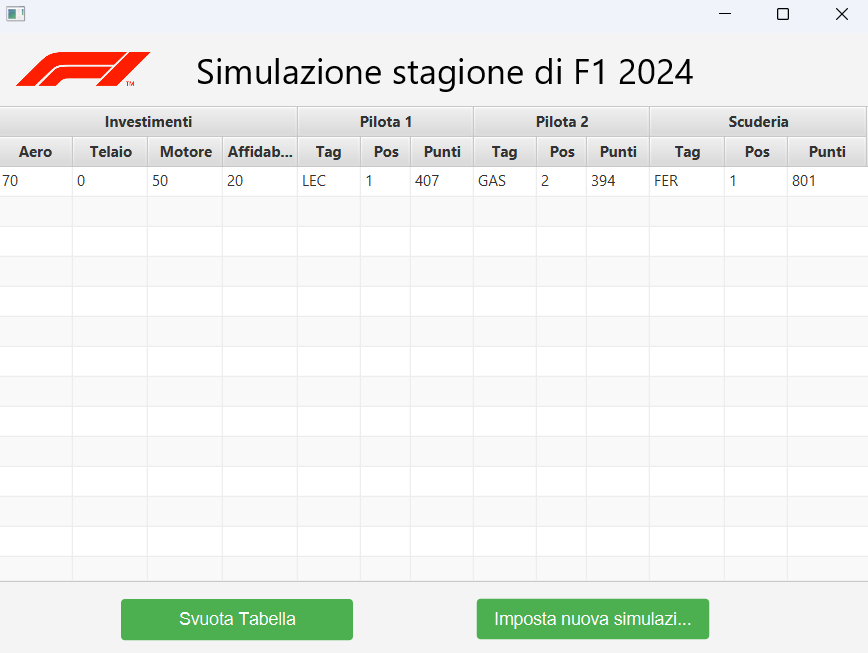
\includegraphics[width=0.8\linewidth]{Figures/singola.png}
    \caption{View Risultati.fxml}
    \label{fig:risultati_fxml}
\end{figure}

Qui sono mostrati i risultati delle varie simulazioni tramite le righe di una tabella. Tramite il pulsante ‘\textit{Avvia nuova simulazione}’ è possibile tornare alla View iniziale e impostare una nuova simulazione. Se la simulazione è stata avviata con successo, nella tabella della View \textit{Risultati.fxml} verrà aggiunta un’altra riga che riporta i dati dell’ultima simulazione. La tabella è in grado di immagazzinare e riportare i risultati di un gran numero di simulazioni, per permettere un semplice e immediato confronto.

Per ogni riga è indicata la scuderia scelta per la simulazione, i valori degli investimenti effettuati, punti e posizioni finali in classifica dei due piloti e della scuderia alla fine dell’anno. Tramite un pulsante ‘\textit{Svuota Tabella}’ è possibile cancellare tutte le righe della tabella.



%\usepackage{amsmath} % Per le formule matematiche
%\usepackage{adjustbox} % Per la gestione delle tabelle

\chapter{Algoritmi e strutture dati}

\section{Struttura del progetto}
L’applicazione, scritta in linguaggio Java, segue il pattern MVC (Model View Controller), quindi divide la struttura software in tre parti principali: model, view e controller. L’applicazione sfrutta il pattern DAO (Database Access Object) che separa la logica di accesso ai dati dalla logica di business.

Il progetto dell’applicazione è disponibile nel repository Github al seguente link: \url{https://github.com/TdP-prove-finali/LapadulaMarioFrancescoPio}.

Il progetto si compone di tre package:
\begin{itemize}
    \item \textbf{db}: contiene le classi utili all’accesso al DB e all’estrazione dei dati;
    \item \textbf{model}: contiene le classi simulative e le classi che definiscono le proprietà degli oggetti utilizzati nella simulazione. Nel model sono memorizzati tutti i dati della simulazione tramite apposite strutture dati;
    \item \textbf{SimulazioneF1}: contiene le classi controller che gestiscono i fogli FXML e, di conseguenza, la GUI (Graphical User Interface).
\end{itemize}

\section{Software utilizzati}
L’applicazione è stata realizzata tramite l’IDE Eclipse. Per la realizzazione di parte dell’interfaccia grafica è stato utilizzato il software SceneBuilder. Il DBMS utilizzato è MariaDB con interfaccia grafica HeidiSQL.

\section{Strutture dati}
La maggior parte dei dati è estratta dal DB e memorizzata in HashMap. Nel model, per la memorizzazione temporanea, sono utilizzati anche LinkedList e ArrayList. Nelle classi dedicate alla simulazione, i tempi in gara e le varie classifiche dei punteggi sono memorizzate e aggiornate tramite HashMap.

\section{Algoritmi simulativi}

\subsection{Simulatore generale}
L’applicazione utilizza un algoritmo di simulazione a eventi discreti. Ci sono tre classi dedicate alla simulazione di eventi: la principale è \texttt{Sim}, che si occupa di amministrare la simulazione dei vari eventi durante l’intera stagione. Durante l’inizializzazione del simulatore principale viene creata una coda di eventi di tipo Sessione. Per ogni circuito presente nella struttura dati fornita, vengono creati due oggetti Sessione: uno di tipo ‘Qualifica’ e uno di tipo ‘Gara’. La classe \texttt{Sim} usa due sottoclassi per simulare nello specifico i vari tipi di eventi: alla classe \texttt{SimQ} sono passate le Sessioni di tipo ‘Qualifica’ e alla classe \texttt{SimR} quelle di tipo ‘Gara’.
\\[3ex]

\begin{figure}[h!]
    \centering
    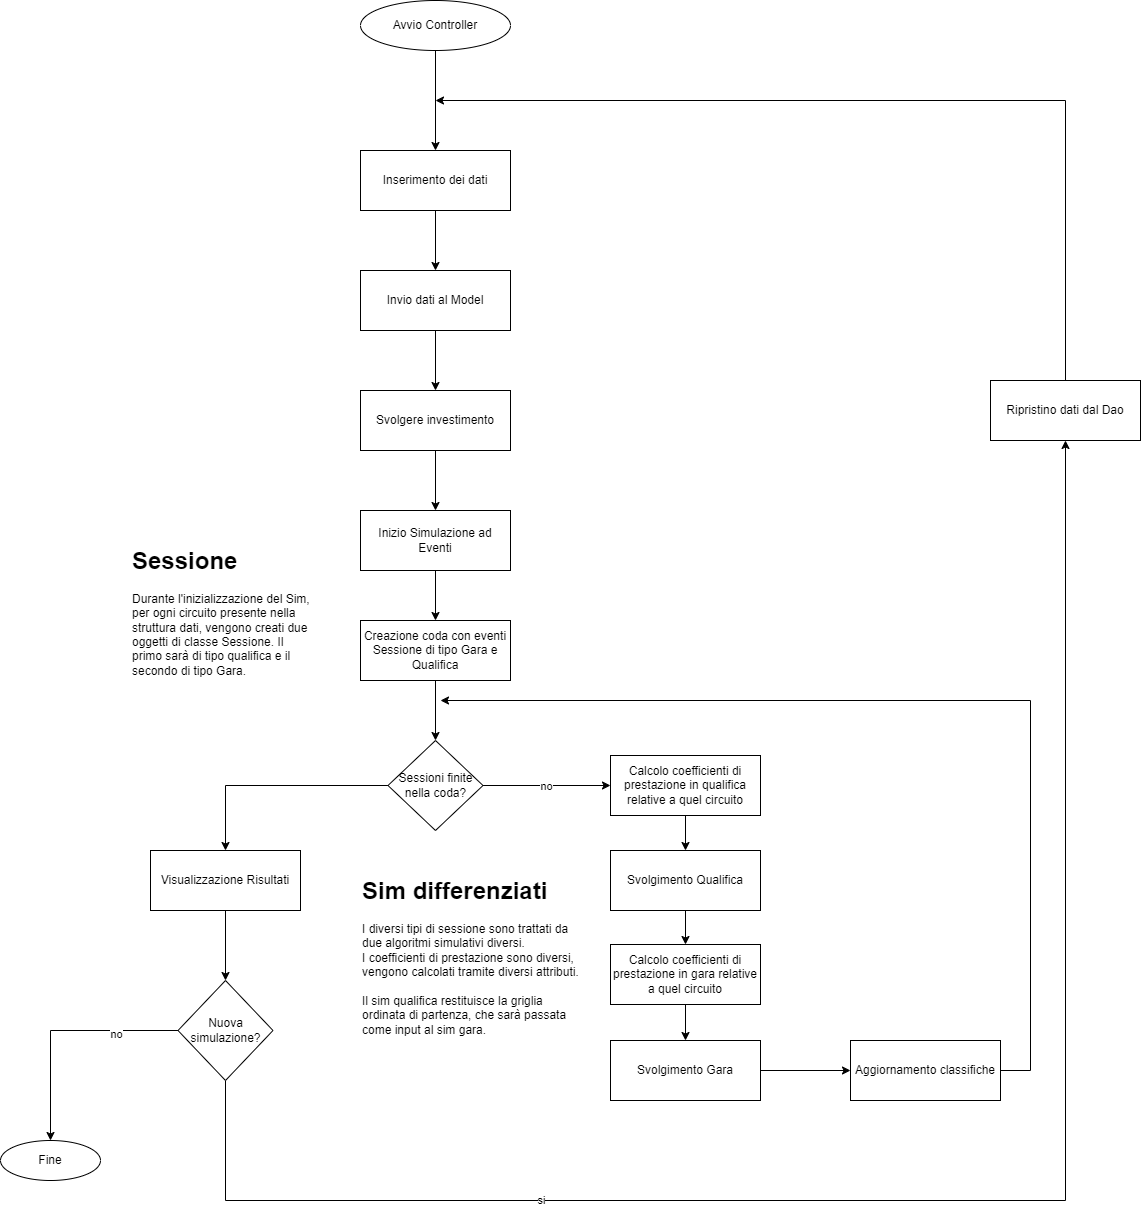
\includegraphics[width=0.8\linewidth, height=11.5cm]{Figures/garaU.png}
    \caption{Flow chart esplicativo riguardo il funzionamento del simulatore generale}
    \label{fig:flowchart_simulatore_generale}
\end{figure}
\newpage
\subsection{Simulatore qualifica}
Alla classe SimQ vengono passati nel costruttore la lista dei piloti partecipanti alla Sessione e l’oggetto Track che indica il circuito su cui viene svolta la sessione.

Il simulatore SimQ ha il compito di calcolare la griglia di partenza per la gara, per poi restituirla alla classe Sim. La griglia viene calcolata confrontando e ordinando degli indici di prestazione relativi ad ogni pilota.

Questi indici sono calcolati all’inizio di ogni sessione attraverso la combinazione dei seguenti fattori:
\begin{itemize}
    \item valore di prestazione della vettura del pilota su quel determinato circuito, calcolato mediante l’algoritmo \texttt{CalcolaPrestazioneScuderia()};
    \item valore di overall totale del pilota;
    \item fattore casuale ottenuto campionando una distribuzione normale.
\end{itemize}

Questi fattori sono poi moltiplicati per delle costanti relative e sommati tra loro per ricavare l’indice di prestazione finale. Successivamente la griglia di partenza viene stilata classificando in ordine decrescente gli indici ottenuti dai piloti.


\subsection{Simulatore gara}
Ricavata la griglia di partenza per la gara, viene fornita al costruttore della classe SimR tramite una lista ordinata di oggetti di tipo Pilota. Prima di iniziare la simulazione delle varie fasi della gara, vi è il calcolo degli indici di prestazione relativi alla gara, diversi da quelli usati nel SimQ per stilare la griglia.

L’indice di prestazione di gara è un valore calcolato attraverso la combinazione dei seguenti fattori:
\begin{itemize}
    \item valore di prestazione della vettura del pilota su quel determinato circuito, calcolato mediante l’algoritmo CalcolaPrestazioneScuderia();
    \item valore di overall totale del pilota;
    \item fattore casuale ottenuto campionando una distribuzione normale;
    \item valore delle caratteristiche Smoothness e Control del pilota moltiplicati per l’indice di consumo gomma in quel circuito;
    \item valore della caratteristica Adaptability del pilota, solo in caso di gara disputata in condizioni di pioggia.
\end{itemize}

Questi fattori sono poi moltiplicati per delle costanti relative e sommati tra loro per ricavare l’indice di prestazione finale. Gli indici saranno poi utilizzati per calcolare il tempo sul giro di un pilota per ogni giro di gara. Calcolati gli indici, si procede simulando il momento della partenza e poi simulando lo svolgimento di ogni giro fino alla fine della gara.

Il tempo di percorrenza di un giro di un pilota è calcolato mediante delle operazioni tra l’indice di prestazione e un fattore casuale campionato da una distribuzione normale.

Durante ogni giro potrebbero capitare imprevisti ad un pilota, come un guasto alla vettura o un incidente in gara, che lo costringerebbero a ritirarsi dalla corsa. L’evento del guasto alla vettura è gestito da un indice di successo probabilistico dipendente dal valore tecnico di Affidabilità della vettura del pilota. Invece l’evento ‘incidente in gara’ è gestito da un indice di successo probabilistico dipendente dalla combinazione dalle caratteristiche Adaptability, Control, Reactions e Aggressivity del pilota.

Prima della fine di ogni giro (dal quarto giro in poi) viene data ai piloti la possibilità di sorpassare se il distacco dal pilota davanti è inferiore a un secondo. In questo caso viene richiamato un algoritmo che stabilirà se il pilota dietro tenterà il sorpasso e se riuscirà nel suo tentativo. Durante un sorpasso, la probabilità che uno o entrambi i piloti coinvolti facciano incidente è più alta della norma e, di conseguenza, che si ritirino dalla gara.

Alla fine di ogni giro vengono poi aggiornati i distacchi tra i piloti in gara. Durante la gara, ogni pilota deve rientrare ai box per un pit stop per due volte. Il tempo perso durante un pit stop viene calcolato tramite operazioni tra i seguenti fattori:
\begin{itemize}
    \item tempo medio di pit stop della scuderia del pilota;
    \item valore qualitativo della Pit Crew della scuderia del pilota;
    \item tempo di percorrenza della pit lane del circuito;
    \item fattore casuale campionato da una distribuzione normale.
\end{itemize}

Per gestire il tempismo dei pit stop, si usa una variabile ‘Stint’ calcolata nel seguente modo:
\[ Stint = \left\lfloor \frac{NGiriGara + 3}{NPitStop + 1} \right\rfloor \]


\begin{figure}[H]
    \centering
    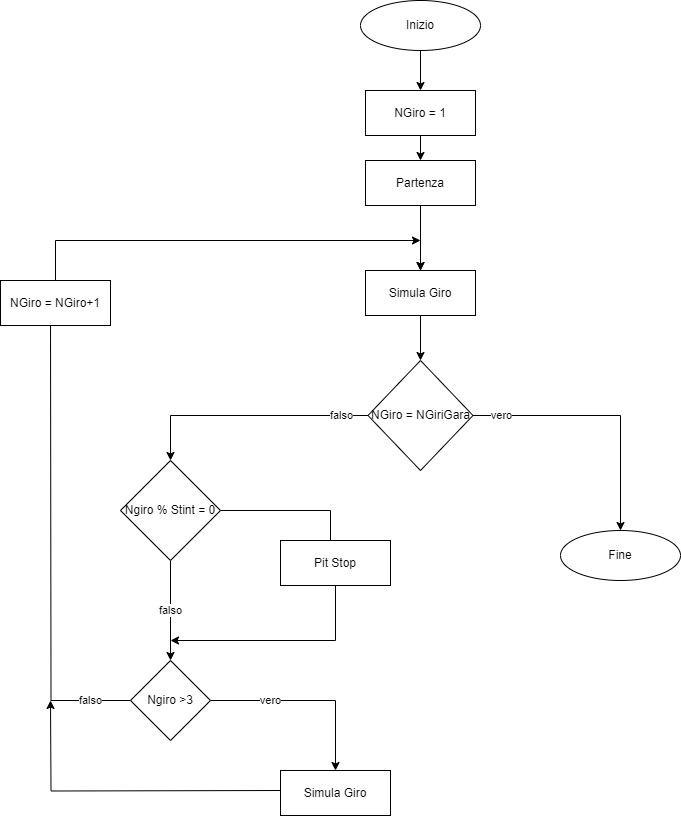
\includegraphics[width=0.8\linewidth, height=9cm]{Figures/gara.png}
    \caption{Flow chart esplicativo riguardo le procedure della simulazione di una gara}
    \label{fig:flowchart_simulatore_gara}
\end{figure}

\subsection{Simulatore sorpasso}
Come riportato nel Capitolo 5.4.3, un sorpasso può verificarsi solo quando il distacco tra due piloti è inferiore a un secondo. L’algoritmo per simulare un sorpasso si divide in due fasi. Un algoritmo preliminare stabilisce in base a un indice di successo probabilistico se il pilota tenterà o meno il sorpasso. Questa variabile dipende dai seguenti fattori:
\begin{itemize}
    \item fattore casuale campionato da una distribuzione normale;
    \item valore della caratteristica Aggressivity del pilota;
    \item indice di probabilità di sorpasso del circuito.
\end{itemize}
Se l’algoritmo restituisce un esito positivo, si aziona un secondo algoritmo che stabilirà l’esito del tentativo di sorpasso. Questo algoritmo prende in analisi le caratteristiche dei due piloti in azione, nello specifico:
\begin{itemize}
    \item overall totale, indice di prestazione della scuderia, valore della caratteristica Defending per il pilota che deve difendersi dal sorpasso; 
    \item overall totale, indice di prestazione della scuderia, valore della caratteristica Overtaking per il pilota che deve effettuare il sorpasso.
\end{itemize}
Questi dati vengono combinati con fattori casuali e poi confrontati per stabilire l’esito della manovra.


\begin{figure}[h!]
    \centering
    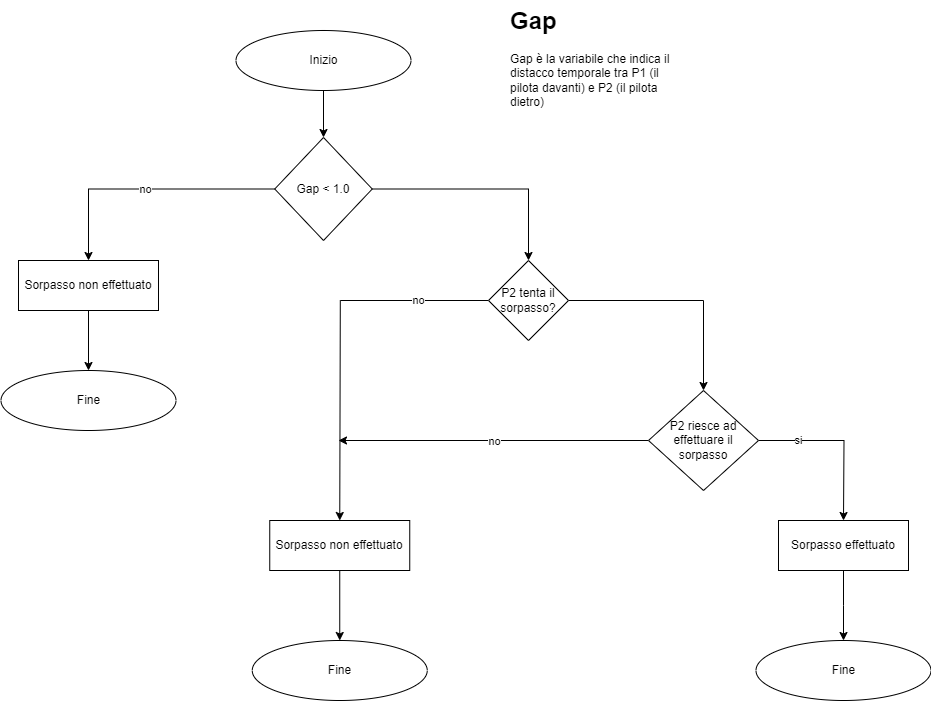
\includegraphics[width=0.8\linewidth]{Figures/Sorpasso1.png}
    \caption{Flow chart esplicativo riguardo il funzionamento dell’algoritmo simulativo per l’azione di sorpasso}
    \label{fig:flowchart_simulatore_sorpasso}
\end{figure}

\subsection{Utilizzo di casualità negli algoritmi}
Nella simulazione sono stati utilizzati fattori randomici per simulare diversi tipi di eventi possibili, come l’azione di sorpasso, la simulazione del tempo sul giro, la partenza della gara, il tempo impiegato per un pit stop e le prestazioni individuali dei piloti in qualifica e in gara. L’utilizzo di questa aleatorietà aiuta a modellare l'incertezza, la variabilità naturale e la complessità di fenomeni che non possono essere descritti completamente da modelli deterministici.



\chapter{Diagramma delle classi}

\section{Package SimulazioneF1}
\vspace{2cm}

\begin{figure}[h!]
    \centering
    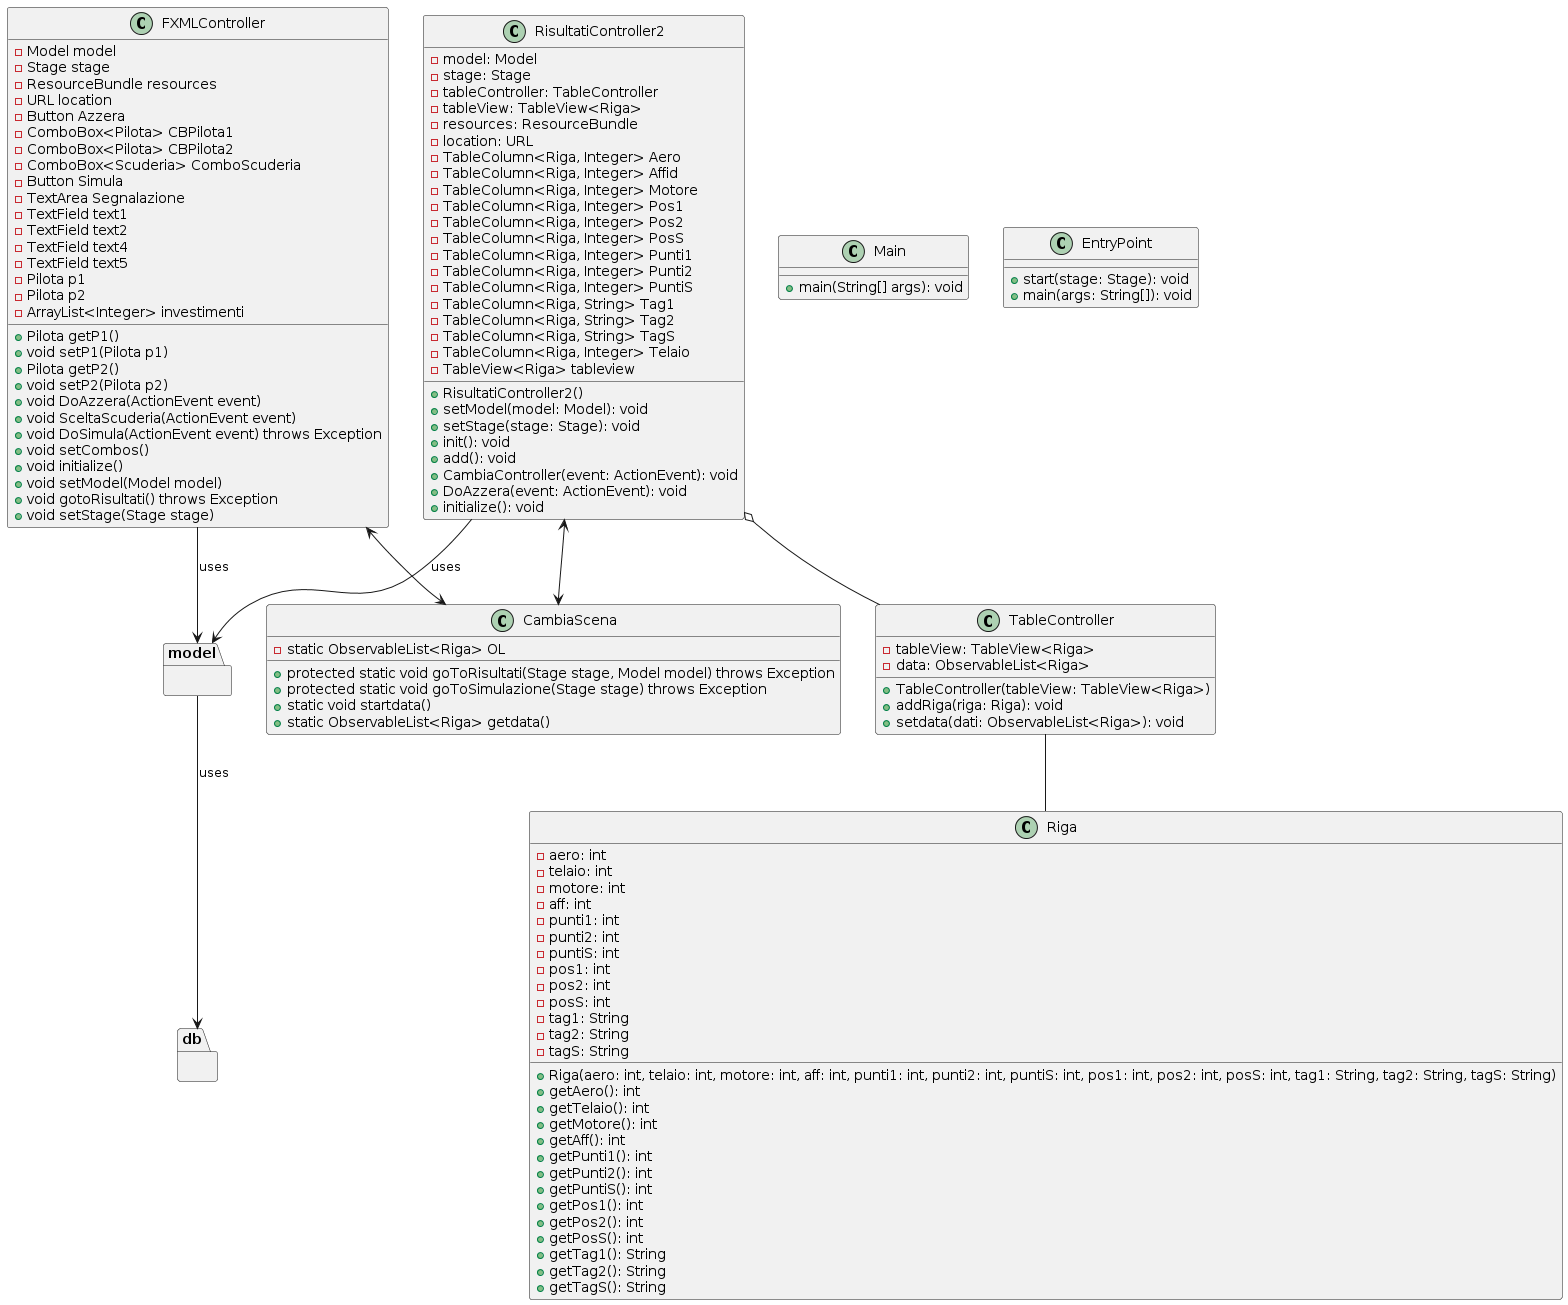
\includegraphics[width=\linewidth]{Figures/uml1.png}
    \caption{Diagramma UML del package SimulazioneF1}
    \label{fig:diagramma_simulazionef1}
\end{figure}
\newpage
\section{Package SimulazioneF1.model}
\vspace{1cm}
\begin{figure}[h!]
    \centering
    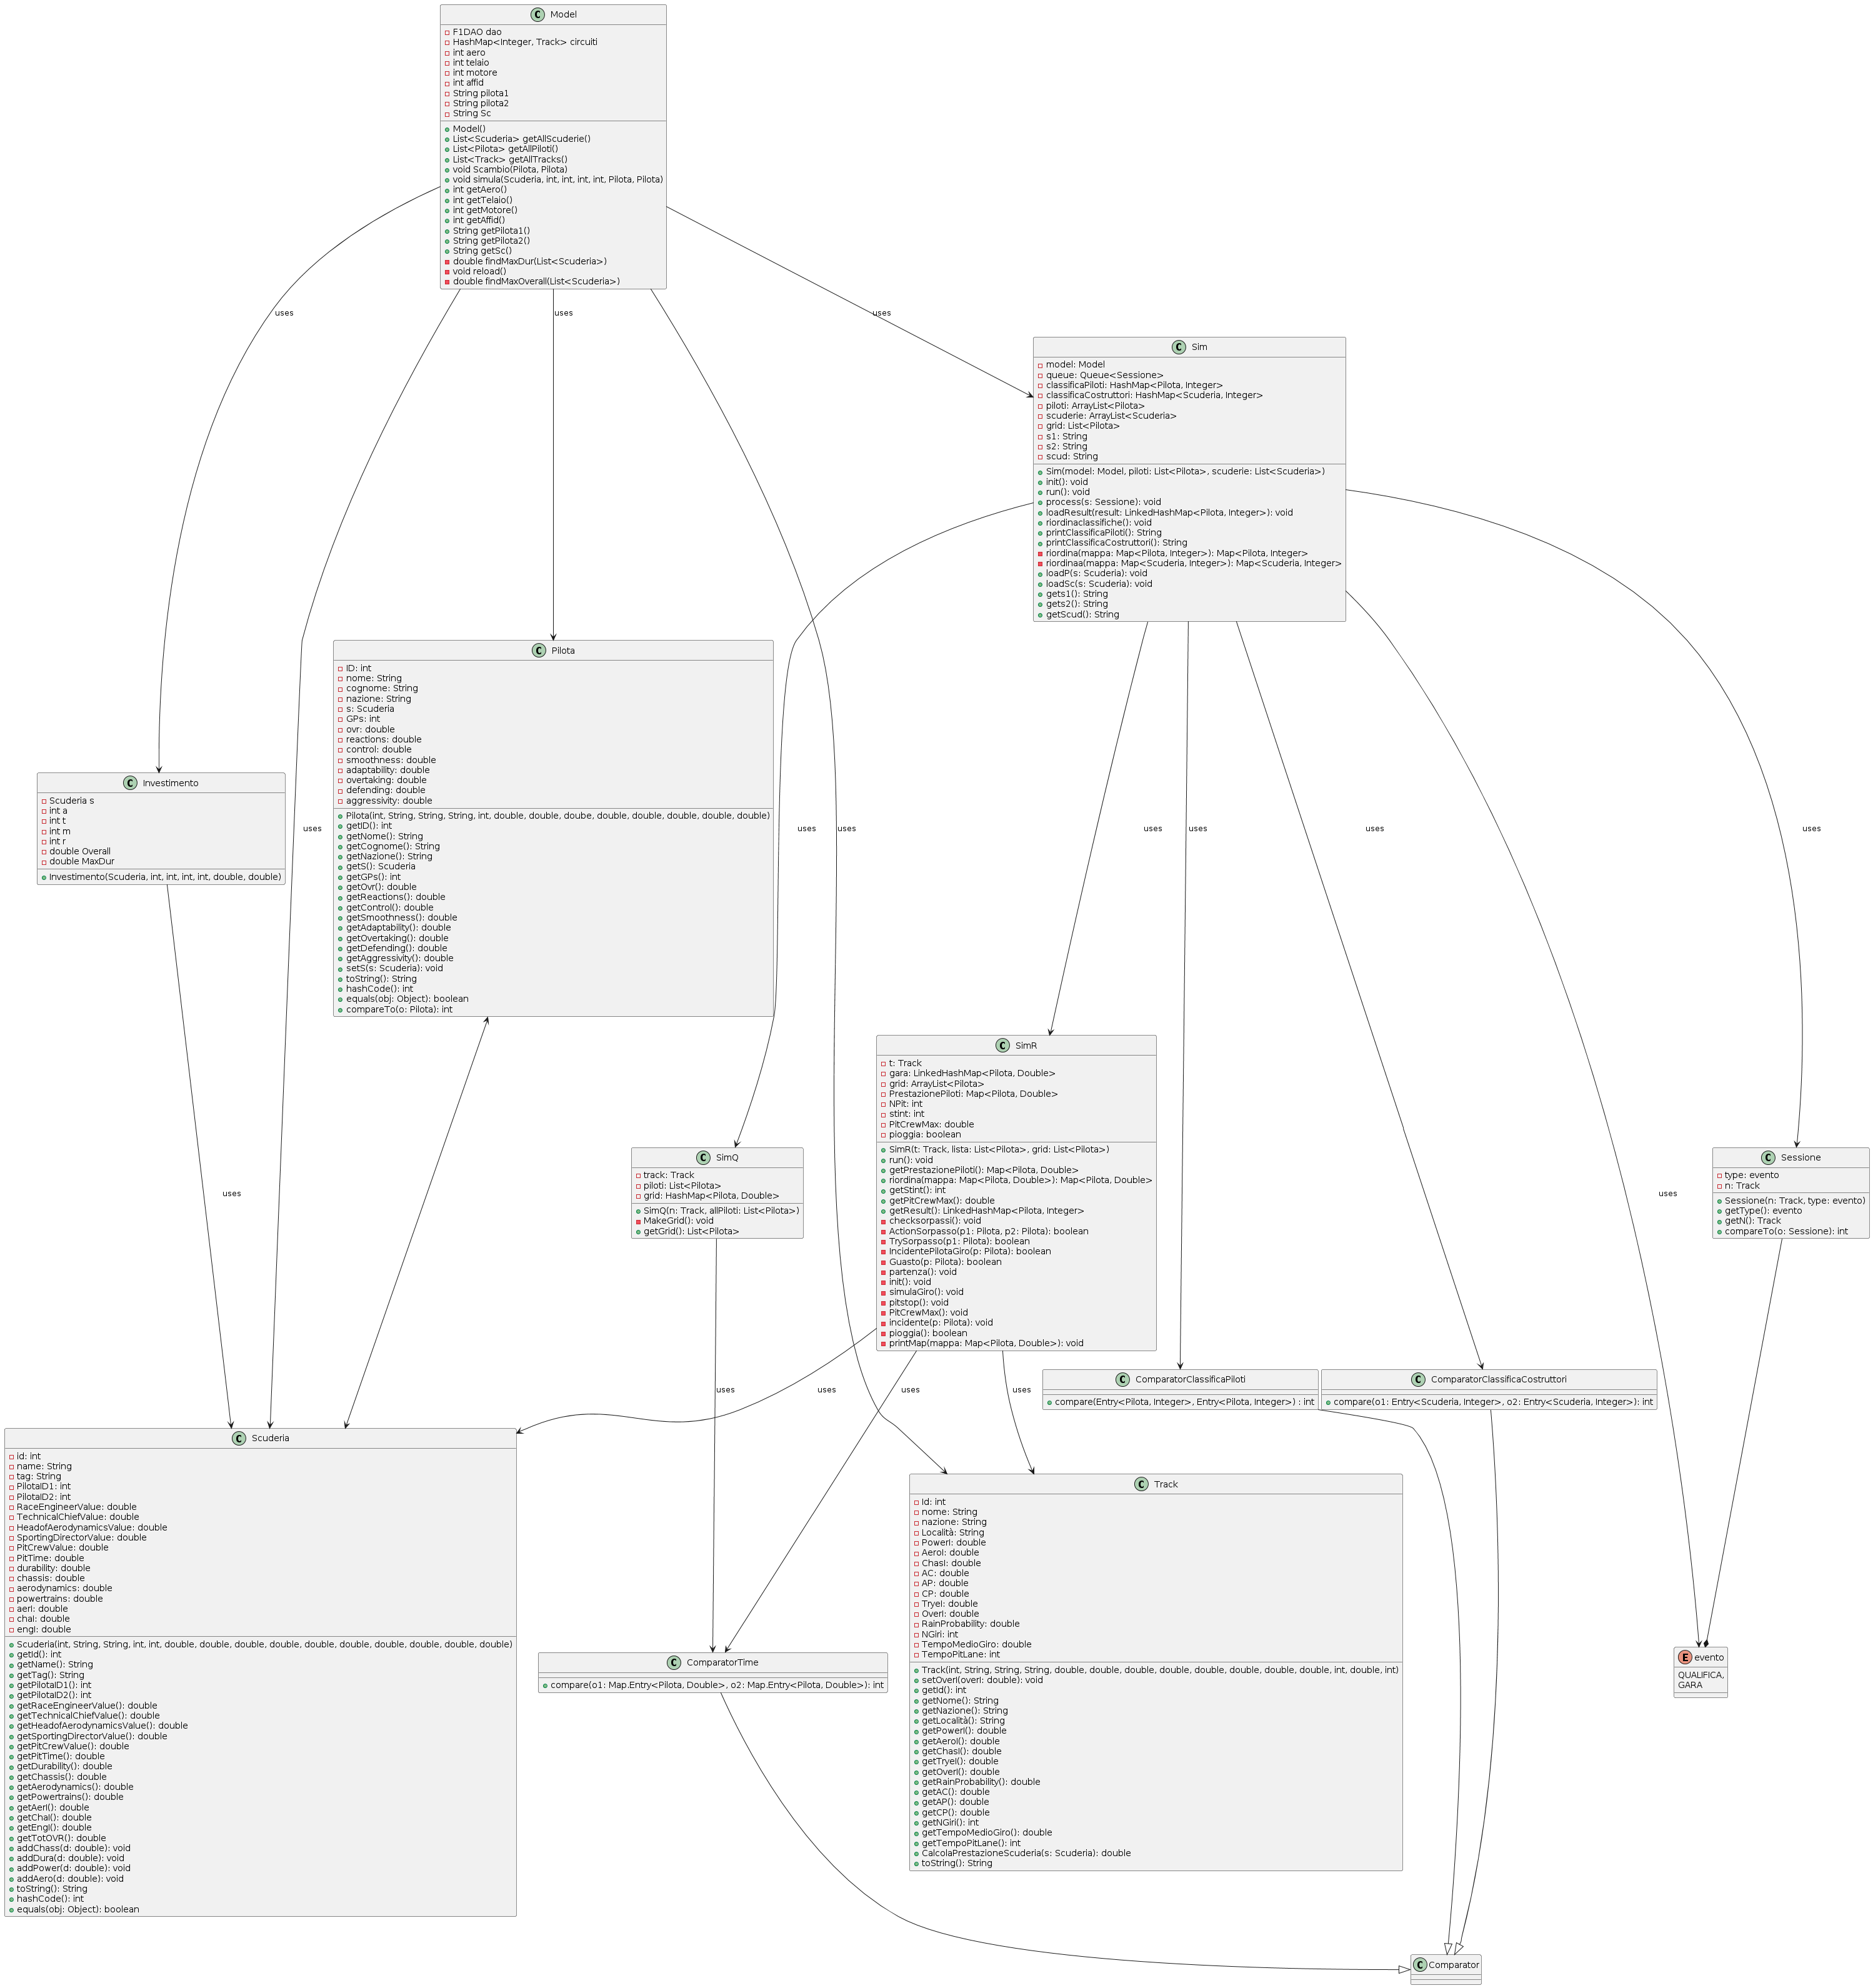
\includegraphics[width=\linewidth, height = 15cm]{Figures/uml3.1.png}
    \caption{Diagramma UML del package SimulazioneF1.model}
    \label{fig:diagramma_model}
\end{figure}
\newpage
\section{Package SimulazioneF1.db}
\vspace{2cm}
\begin{figure}[h!]
    \centering
    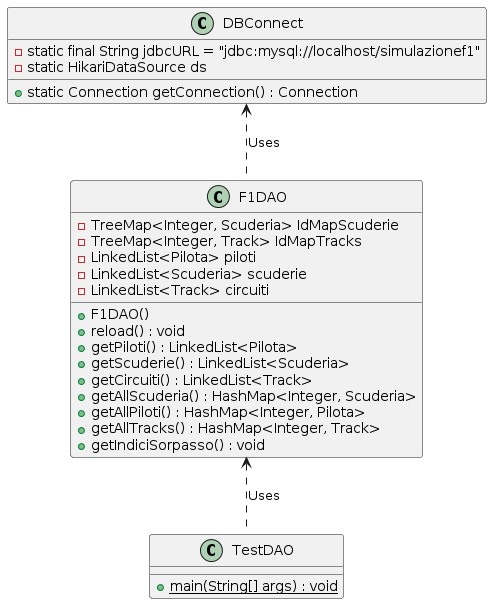
\includegraphics[width=0.8\linewidth]{Figures/uml2.png}
    \caption{Diagramma UML del package SimulazioneF1.db}
    \label{fig:diagramma_db}
\end{figure}



\chapter{Schermate dell'applicazione}

\counterwithout{figure}{chapter}
\counterwithout{table}{chapter}
\counterwithin{figure}{chapter}
\counterwithin{table}{chapter}

\begin{figure}[h!]
    \centering    
        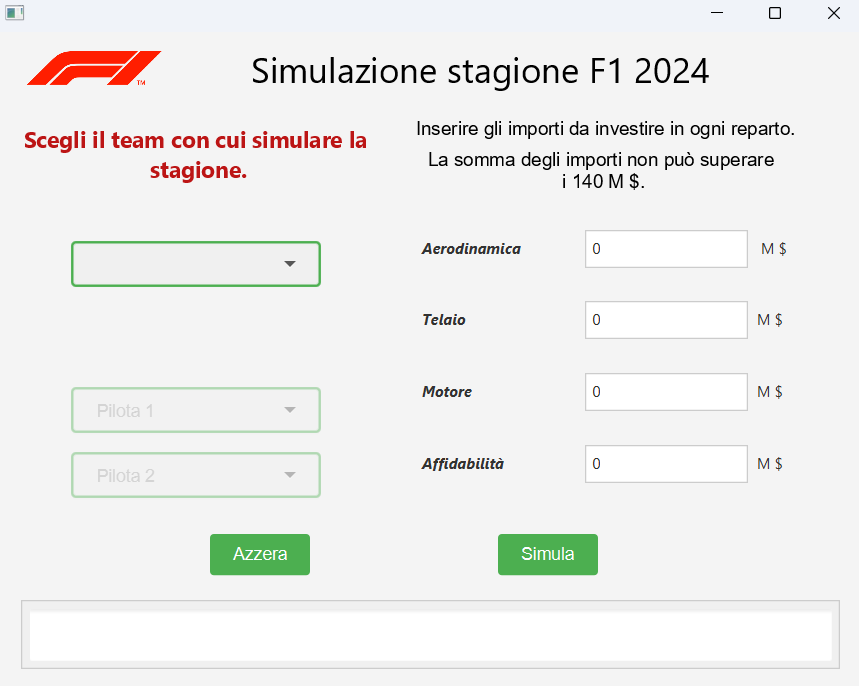
\includegraphics[width=\textwidth]{Figures/schermata1.png}
        \caption{Schermata di simulazione vuota}
        \label{fig:schermata_simulazione_vuota}
\end{figure}
\begin{figure}[h!]
        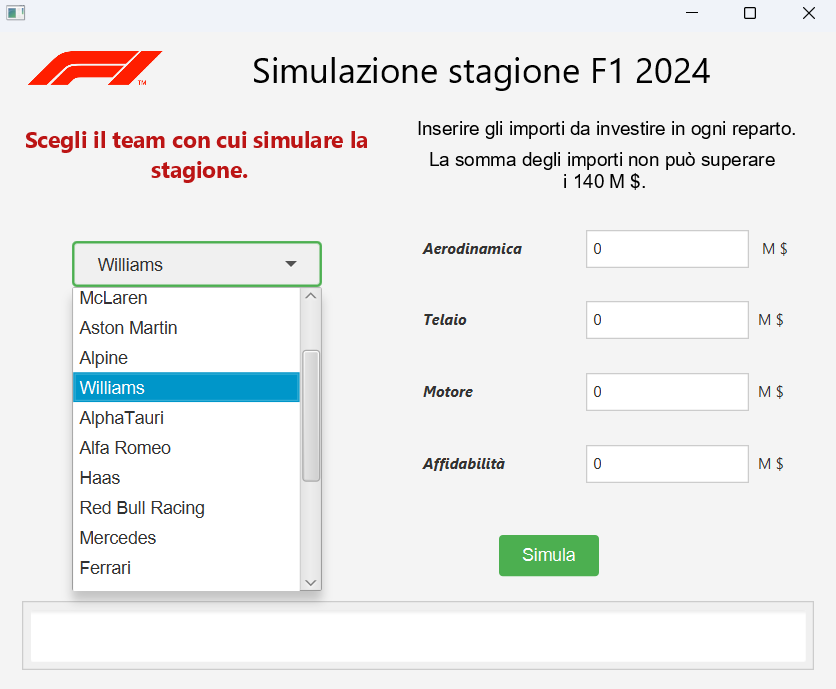
\includegraphics[width=\textwidth]{Figures/schermata2.png}
        \caption{Selezionamento della scuderia tramite la ComboBox}
        \label{fig:selezionamento_scuderia}
\end{figure}

\begin{figure}[h!]
    \centering
    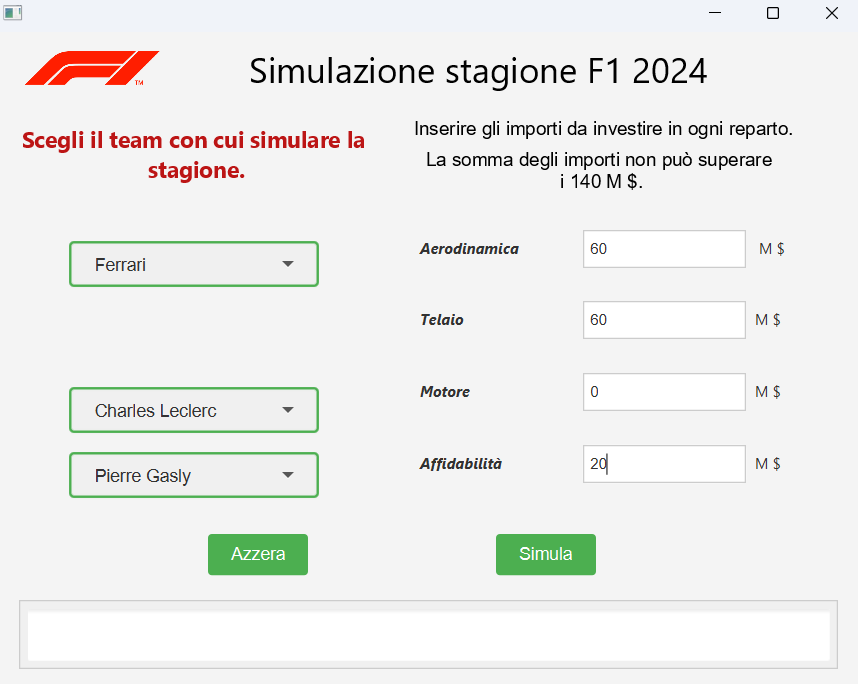
\includegraphics[width=\textwidth]{Figures/schermata3.png}
    \caption{Schermata di simulazione con i parametri impostati correttamente}
    \label{fig:schermata_simulazione_parametri}
\end{figure}

\begin{figure}[h!]
    \centering
        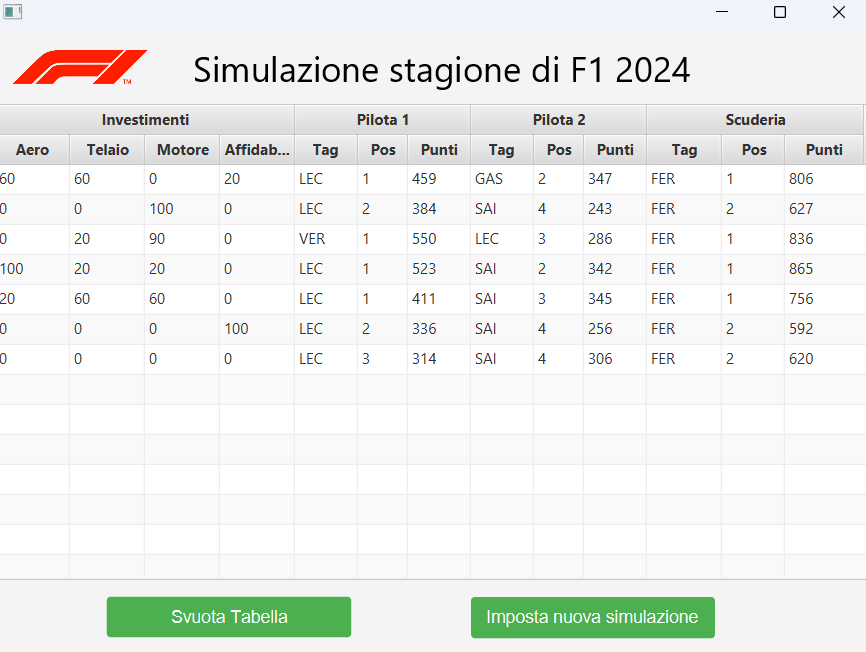
\includegraphics[width=\textwidth]{Figures/schermata4.png}
        \caption{Tabella riepilogativa con i risultati delle simulazioni svolte con un solo team}
        \label{fig:tabella_riepilogativa_singolo_team}
    \hspace{1cm}
        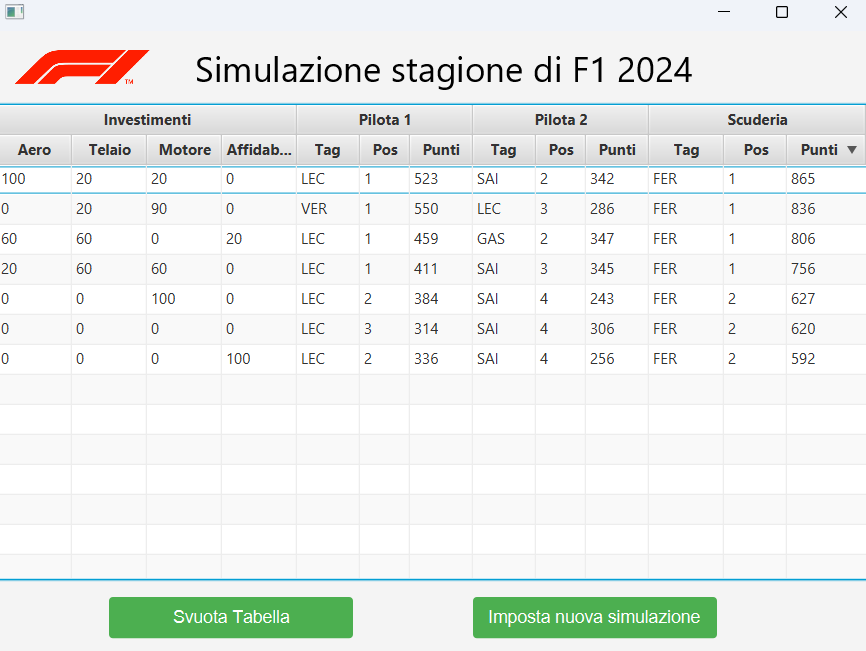
\includegraphics[width=\textwidth]{Figures/ordinata.png}
        \caption{Tabella riepilogativa ordinata in base al punteggio finale nella classifica costruttori}
        \label{fig:tabella_riepilogativa_ordine_punteggio}
\end{figure}

\begin{figure}[h!]
    \centering
    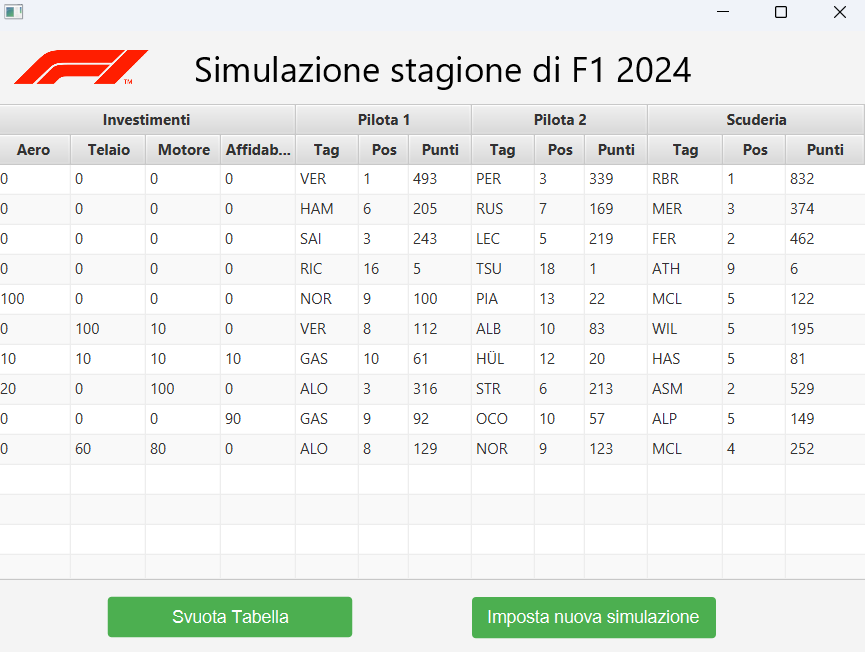
\includegraphics[width=\textwidth]{Figures/schermata5.png}
    \caption{Tabella riepilogativa con i risultati delle simulazioni svolte con diversi team}
    \label{fig:tabella_riepilogativa_diversi_team}
\end{figure}



\counterwithin{figure}{section}
\chapter{Risultati sperimentali e analisi}

\section{Parametri utilizzati}
Sono state effettuate simulazioni prendendo in esame 4 delle 10 scuderie disponibili. In tre di queste l’obiettivo è quello di individuare il miglior asset di investimento, nella quarta invece è quello di analizzare quanto l’introduzione di un nuovo pilota possa incidere sul risultato finale. 
Per le prime tre simulazioni, per ognuno dei team, sono stati utilizzati 27 diversi asset (Figura~\ref{fig:asset}) di investimenti per la comparazione. 
 
\begin{figure}[H]
    \centering
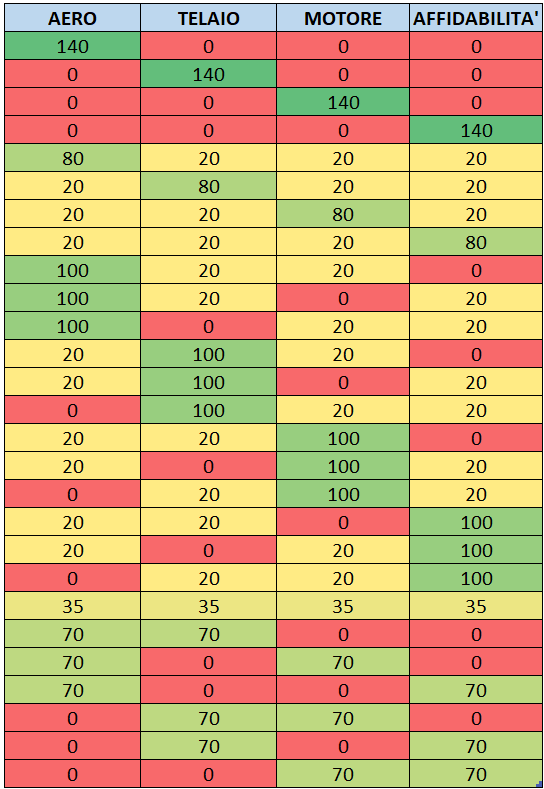
\includegraphics[width=0.7\textwidth, height=9.6cm]{Figures/asset.png} 
    \caption{Tabella degli asset scelti per svolgere le simulazioni}
    \label{fig:asset}
\end{figure}

La tabella in Figura~\ref{fig:asset} utilizza una codifica che utilizza un gradiente di colori per rappresentare i valori numerici e facilitare l'interpretazione visiva dei dati, permettendo di identificare rapidamente i valori più significativi. La legenda dei colori è la seguente:
\begin{itemize}
    \item Verde : Valori alti;
    \item Giallo : Valori bassi;
    \item Rosso : Valori nulli.
\end{itemize}
Questa codifica facilita l'interpretazione visiva dei dati, permettendo di identificare rapidamente i valori più significativi.

\newpage

\section{Variabilità dei dati}
Inoltre, al fine di ridurre l'influenza della variabilità delle singole simulazioni, ogni asset viene valutato sulla base della media di due simulazioni indipendenti.

È importante sottolineare che le simulazioni possono mostrare risultati significativamente diversi anche quando vengono eseguite con gli stessi parametri in input, a causa delle molte variabili casuali coinvolte nel processo.

A titolo esemplificativo, sono state condotte 20 simulazioni utilizzando gli stessi parametri di input per la Scuderia Ferrari.
 
\begin{figure}[h]
    \centering
    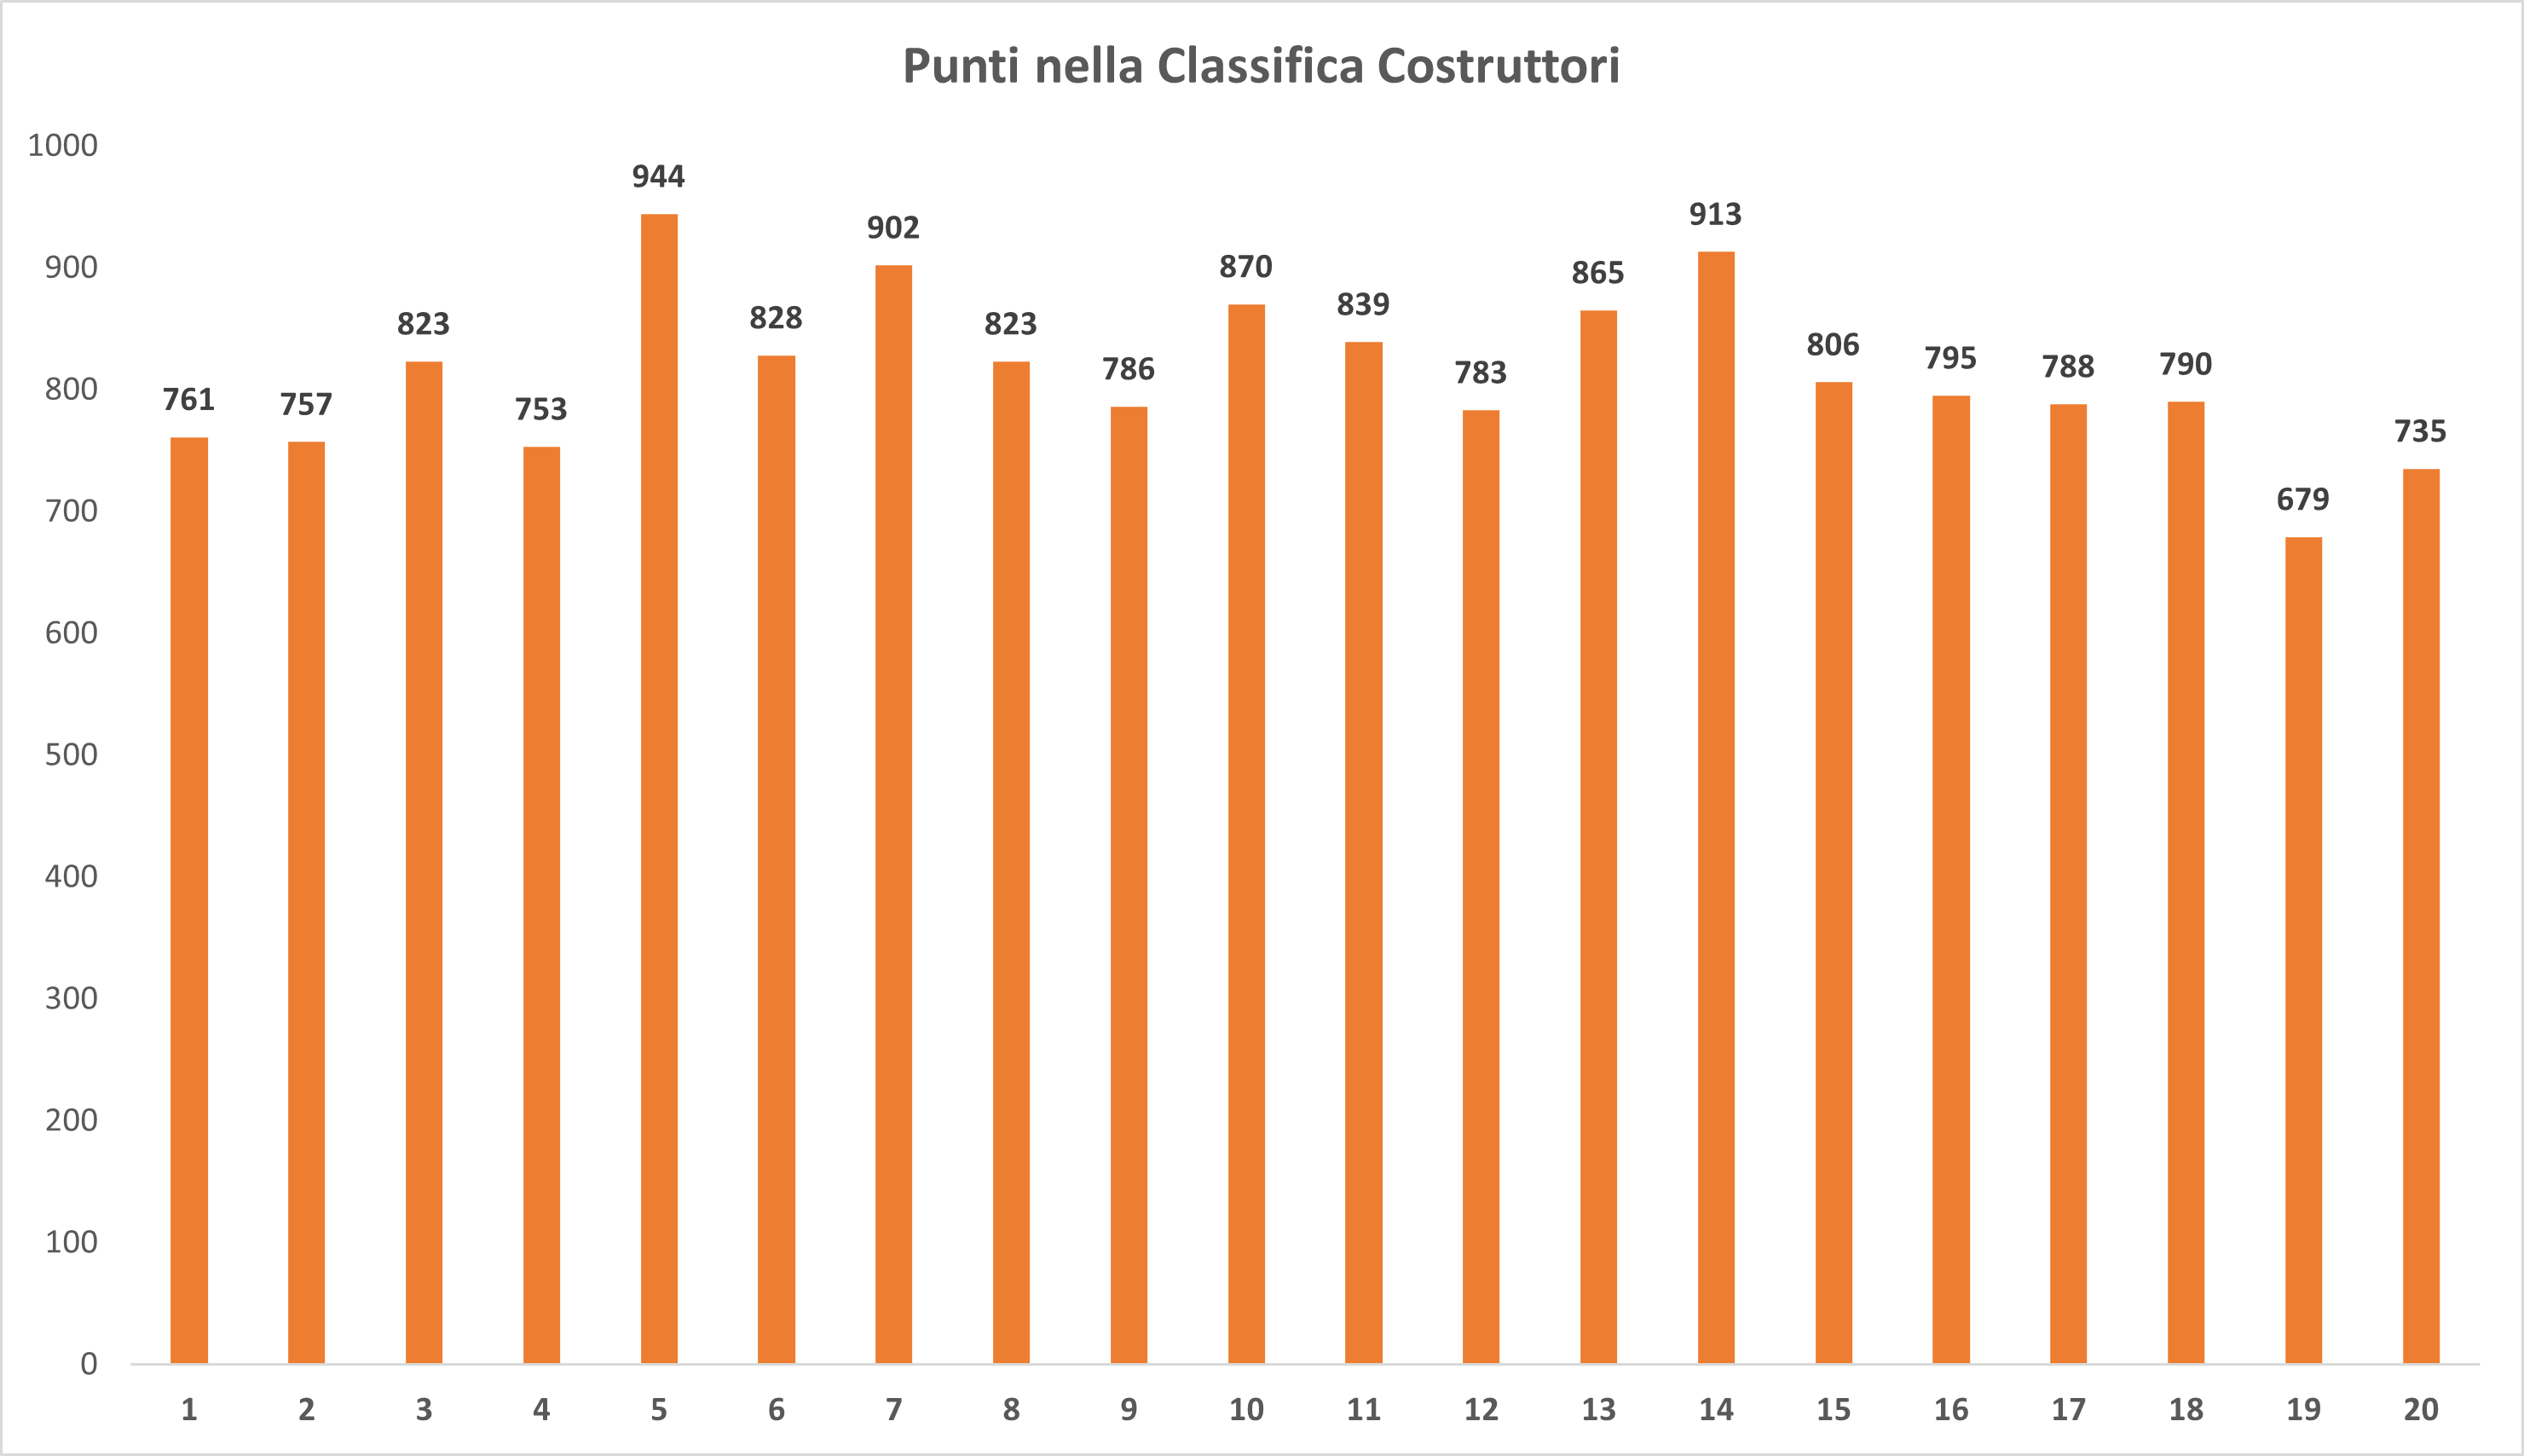
\includegraphics[width=\textwidth]{Figures/fvar.png}
    \caption{Grafico a barre dei risultati della simulazione con Scuderia Ferrari utilizzando lo stesso asset di investimenti}
    \label{fig:ferrari}
\end{figure}

I risultati numerici delle 20 simulazioni costituiscono una popolazione di campioni. Tra questi, il valore massimo ottenuto è stato di 944 punti, mentre il valore minimo è stato di 679 punti, con una differenza di 265 punti tra i due estremi.

La media dei risultati ottenuti è stata di 812 punti, con una deviazione standard\footnote{dettagli aggiuntivi nell'Appendice~\ref{appendice:ds}} di 64.38 punti e un coefficiente di variabilità\footnote{dettagli aggiuntivi nell'Appendice~\ref{appendice:cv}} del 8%.

Questi dati evidenziano una variabilità significativa nei risultati delle simulazioni, anche quando vengono utilizzati gli stessi parametri di input.



\newpage
\section{Simulazione Ferrari}

\begin{figure}[h]
    \centering
    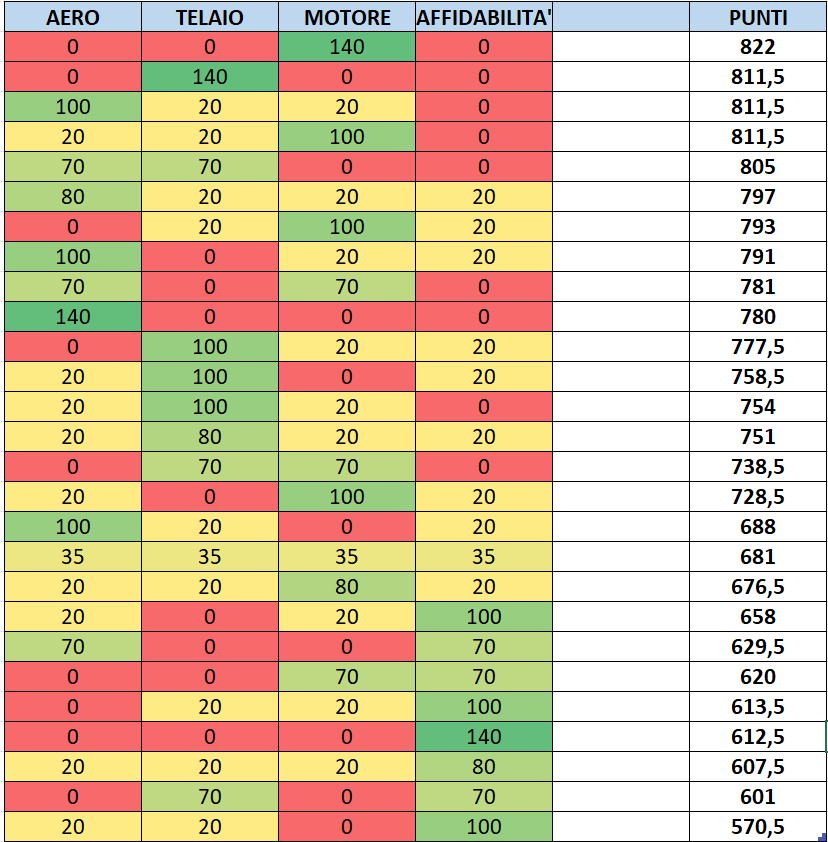
\includegraphics[width=\textwidth, height=11cm]{Figures/ferrari1.png} 
    \caption{Tabella che riporta i risultati della simulazione con la Scuderia Ferrari usando i 27 diversi asset di investimento}
    \label{fig:ferrari_assets}
\end{figure}

Dai risultati riportati nella Figura~\ref{fig:ferrari_assets}, si osserva che il massimo punteggio raggiungibile per il team Ferrari si aggira attorno agli 800 punti. Guardando le migliori cinque simulazioni, emerge chiaramente che un investimento nel settore dell’Affidabilità non è vantaggioso per il team. La tabella mostra una distribuzione prevalentemente negativa (cellule verdi in basso), indicando risultati inferiori.

Escluso il settore dell’Affidabilità, gli altri tre sembrano poter incidere in maniera simile sul risultato finale, ma tramite il calcolo del IPCI\footnote{dettagli aggiuntivi nell'Appendice~\ref{appendice:ipci}}(Figura~\ref{fig:ipci}) si intuisce come l’ambito Telaio sia leggermente meno significativo degli altri due. 


\begin{figure}[h]
    \centering
    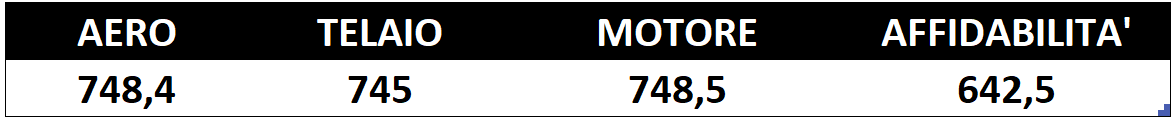
\includegraphics[width=\textwidth]{Figures/ferrari2.png} % sostituire con il nome del file immagine
    \caption{Tabella che riporta il valore IPCI dei vari reparti in cui è possibile investire con la scuderia Ferrari}
    \label{fig:ipci}
\end{figure}

In conclusione, le migliori strategie per il team Ferrari sembrano essere due: investire la totalità del budget nel settore motoristico o ripartire le risorse tra le tre aree Telaio, Motore e Aerodinamica.

\newpage

\section{Simulazione Alpine}

\begin{figure}[h]
    \centering
    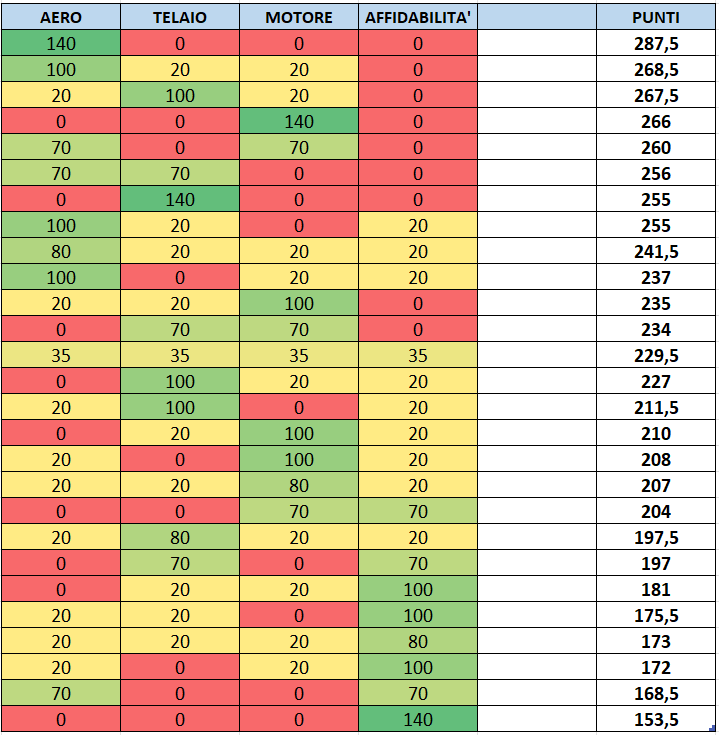
\includegraphics[width=\textwidth, height = 11cm]{Figures/alpine1.png}
    \caption{Tabella dei risultati della simulazione con la Scuderia Alpine usando i 27 diversi asset di investimento}
    \label{fig:figura9_5}
\end{figure}

\begin{figure}[h]
    \centering
    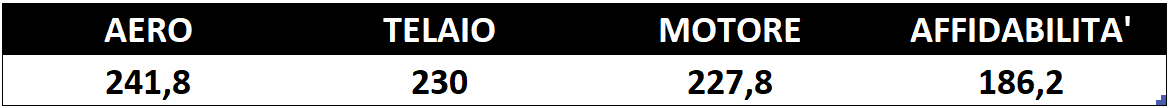
\includegraphics[width=\textwidth]{Figures/alpine2.png}
    \caption{Tabella del valore IPCI dei vari reparti in cui è possibile investire con la Scuderia Alpine}
    \label{fig:figura9_6}
\end{figure}

Dai risultati riportati nella Figura~\ref{fig:figura9_5} è facile notare quanto un investimento nel settore dell’affidabilità sia poco producente in termini di punti nella classifica finale. Infatti, le migliori sette simulazioni riportate indicano un investimento nullo in tale settore.

Per quanto riguarda gli altri tre settori, tramite una semplice analisi visiva della Figura~\ref{fig:figura9_5} si potrebbe intuire che ce ne sia uno più vantaggioso di altri in cui investire: quello Aerodinamico. Ciò è confermato anche dal confronto dei valori di IPCI\footnote{dettagli aggiuntivi nell'Appendice~\ref{appendice:ipci}} (Figura~\ref{fig:figura9_6}): il settore dell’Aerodinamica ha più di 11 punti rispetto a Telaio e Motore, che risultano essere comparabili in termini di rendimento.

Si evince quindi che la miglior strategia di investimento per il team Alpine sia quella di investire la totalità del budget o quasi nel settore dell’aerodinamica. Questa strategia permetterebbe al team di raggiungere un punteggio che si aggira intorno ai 290 punti.

\newpage

\section{Simulazione Haas}

\begin{figure}[h]
    \centering
    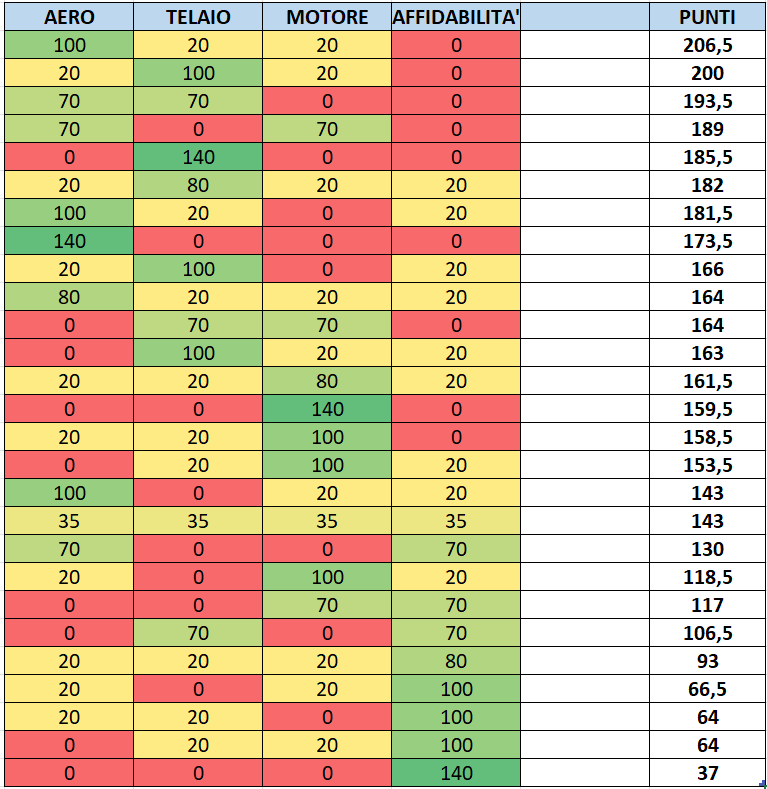
\includegraphics[width=\textwidth, height=11cm]{Figures/haas1.png}
    \caption{Tabella dei risultati della simulazione con la Scuderia Haas usando i 27 diversi asset di investimento}
    \label{fig:figura9_7}
\end{figure}

Per quanto riguarda la scuderia Haas, dall’analisi della tabella mostrata in Figura~\ref{fig:figura9_7}, si riconferma il fatto che un investimento nell’affidabilità non è fruttuoso. Del resto, dal confronto tra le varie aree si può notare come la distribuzione dei colori nella tabella indichi che un investimento nel settore Motore sia meno vantaggioso che nei settori Aerodinamica e Affidabilità. Infatti, confrontando i valori di IPCI\footnote{dettagli aggiuntivi nell'Appendice~\ref{appendice:ipci}} si nota come Aerodinamica e Telaio abbiano un punteggio molto simile e il settore del Motore sia staccato di circa 16 punti. Fanalino di coda l’Affidabilità, lontana dai punteggi degli altri settori.

\begin{figure}[h]
    \centering
    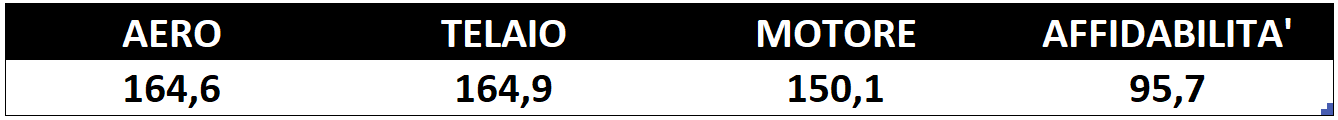
\includegraphics[width=\textwidth]{Figures/haas2.png}
    \caption{Tabella del valore IPCI dei vari reparti in cui è possibile investire con la scuderia Haas}
    \label{fig:figura9_8}
\end{figure}

Dai dati ricavati dalle varie simulazioni si giunge alla conclusione che la miglior strategia d’investimento per il team Haas è quella di concentrare l’intero budget tra i settori di Aerodinamica e Telaio.

\newpage

\section{Analisi Aston Martin}

In questa simulazione non sono stati apportati investimenti tecnici al team ma è stato sostituito un pilota del team, Lance Stroll (dodicesimo pilota per overall), con Max Verstappen (primo pilota per overall). Sono state effettuate 15 simulazioni per coppia di piloti:
\begin{itemize}
    \item Coppia standard: Fernando Alonso – Lance Stroll;
    \item Coppia sperimentale: Fernando Alonso – Max Verstappen.
\end{itemize}




\begin{figure}[h]
    \centering
    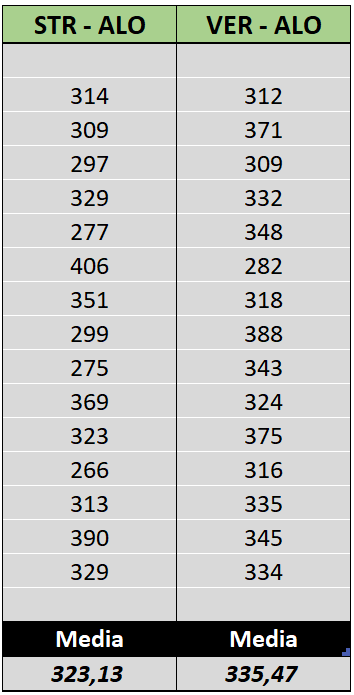
\includegraphics[width=0.5\textwidth, height = 9cm]{Figures/piloti.png}
    \caption{Tabella che riporta il confronto dei risultati delle simulazioni della Scuderia Aston Martin con una diversa coppia di piloti}
    \label{fig:figura9_9}
\end{figure}

Nonostante una netta differenza tra overall tra Max Verstappen (90,75) e Lance Stroll (83,05), i risultati finali non discostano di molto. La media dei punteggi ottenuti dimostra che a fronte di un cambio pilota che ha apportato un incremento di 8.7 nell’overall del pilota, il punteggio finale nella classifica costruttori è aumentato solo di 12,34 punti in media. Quindi la sostituzione del pilota Lance Stroll con il pilota più abile Max Verstappen non risulta essere particolarmente significativa per la classifica finale della scuderia Aston Martin.

\newpage

\section{Analisi finale}

In conclusione, un’osservazione ricorrente nelle prime tre simulazioni è che un investimento nel settore legato all’Affidabilità non ha un buon ritorno in termini di punti nella classifica costruttori, soprattutto per i team nella parte bassa della classifica. I dati evidenziano che è più vantaggioso concentrarsi sullo sviluppo dei settori che migliorano le prestazioni andando a ridurre i tempi sul giro, piuttosto che sviluppare un settore che mitiga i rischi legati ai guasti tecnici e che costringerebbero la vettura al ritiro. Relativamente agli altri settori, la strategia varia significativamente da scuderia a scuderia, poiché ciascuna ha un bilanciamento unico tra i reparti tecnici. Sebbene le tre simulazioni abbiano mostrato che l’Aerodinamica tende a garantire un buon tasso di rendimento, è importante notare che questa osservazione potrebbe non essere universalmente valida per tutte le dieci scuderie. Le simulazioni effettuate utilizzando un ampio numero di asset hanno permesso di individuare strategie particolarmente fruttuose per i team presi in considerazione. Tuttavia, per aumentare l'efficacia della ricerca, sarebbe necessario esplorare un numero molto maggiore di combinazioni di investimento e condurre simulazioni più approfondite per ciascuna di esse, al fine di ridurre la variabilità degli output e ottenere risultati più solidi e generalizzabili. Per quanto riguarda l’opportunità di poter cambiare i piloti della propria squadra, si è osservato che nel caso di Aston Martin, nonostante una sostituzione importate, non si è registrato un gran incremento di punti nella classifica finale. Al fine di valutare al meglio quanto un cambio pilota possa influire sul punteggio finale di una scuderia, è necessario effettuare simulazioni con diverse scuderie, soprattutto quelle posizionate nella parte bassa della classifica che potrebbero avere valori tecnici simili tra loro.









\chapter{Conclusioni e Miglioramenti}

In sintesi, l’applicazione si dimostra efficace nel raggiungere l’obiettivo di simulare vari scenari della stagione 2024 di F1. La complessità degli eventi simulati è stata attentamente considerata, integrando una vasta gamma di fattori probabilistici e casuali che riflettono l'imprevedibilità caratteristica della competizione tra piloti su differenti vetture da corsa.

Per quanto riguarda l’User Experience, l'interfaccia è stata progettata per offrire un'interazione fluida e intuitiva. A tal proposito la seconda View (Figura \ref{fig:risultati_fxml}) della GUI(Graphical User Interface) è stata specificamente concepita per consentire un rapido confronto tra i risultati ottenuti, ottimizzando i tempi di elaborazione per garantire una fruizione immediata dei dati finali.

Una delle caratteristiche fondamentali del programma è la sua capacità di non diventare obsoleto nel tempo. Grazie all'importazione di dataset aggiornati sulla qualità delle vetture e dei piloti, l'applicazione è pronta ad essere utilizzata anche per le future stagioni di Formula 1, mantenendo la sua rilevanza e precisione nel tempo.

Nonostante l'attuale efficacia del programma, la ricerca della soluzione ottimale per il bilanciamento degli investimenti tecnici rimane un obiettivo complesso. Le simulazioni condotte finora hanno evidenziato l'importanza di eseguire centinaia di iterazioni per esplorare tutte le principali combinazioni di investimento e limitare la variabilità intrinseca alle simulazioni.

Inoltre, vi sono altri fattori strutturali che potrebbero migliorare ulteriormente l'applicazione, modellando più accuratamente il singolo evento gara e lo sviluppo stagionale. Questi sono:
\begin{itemize}[label=-]
    \item Strategia di gara: questa potrebbe essere implementata attraverso un algoritmo di machine learning. La strategia di gara è solitamente calcolata in base ad informazioni sulle telemetrie, temperature del circuito, stato degli pneumatici, posizioni di partenza, tipologia di circuito e condizioni meteo. Esse sono differenziate per i vari piloti in pista e a volte possono ribaltare l’esito della gara.
    \item Usura delle gomme: questo fattore è molto influente in F1 poiché va ad influenzare la strategia di gara e influisce molto nelle fasi finali della gara. Il coefficiente di usura della gomma è un parametro difficile da calcolare poiché dipende dalla vettura, dalla capacità del pilota, dall’asfalto e dalle temperature.
    \item Sviluppo di tutti i team: la simulazione non tiene conto del fatto che durante la stagione anche gli altri team possono investire per migliorare la qualità della vettura. Inoltre, nel contesto reale della Formula 1 gli investimenti non avvengono totalmente agli inizi della stagione, bensì gradualmente durante il susseguirsi delle gare.
    \item Successo di un investimento: non sempre un investimento porta notevoli migliorie tecniche alla vettura. Può succedere che un investimento su una specifica area abbia un tasso di rendimento molto basso. Questo si potrebbe modellare con l’aggiunta di variabili probabilistiche legate alla qualità del reparto di ricerca del team.
\end{itemize}

Inoltre è molto importante sottolineare che i dati presenti nel database derivano da stime effettuate da enti legati alla Formula 1 e non rappresentano la qualità effettiva delle vetture dei team, dal momento che questi dati vengono tenuti segreti dalle scuderie. L'assenza di dati dettagliati e aggiornati implica quindi una certa incertezza nei risultati predetti dall'applicazione.

In conclusione, nonostante le sfide e le limitazioni attuali, l'applicazione rappresenta un valido strumento di supporto per la pianificazione degli investimenti di un team di Formula 1. Potrebbe altresì costituire una solida base per lo sviluppo di videogiochi manageriali dedicati al campionato di Formula 1, ampliando così il suo potenziale utilizzo nel settore dell'intrattenimento e della simulazione sportiva.




\appendix
\chapter{Formule matematiche}

\section*{Deviazione standard}
\label{appendice:ds}
La deviazione standard, o scarto quadratico medio, è un indice di dispersione statistica, vale a dire un indicatore usato per fornire una stima sintetica della variabilità di una popolazione di dati o di una variabile casuale. 

\[ \sigma_X = \sqrt{\frac{1}{N} \sum_{i=1}^{N} (x_i - \mu_X)^2}, \]

In statistica descrittiva, lo scarto quadratico medio di un carattere \( X \) rilevato su una popolazione di \( N \) unità statistiche si definisce nel seguente modo:
\begin{itemize}
    \item \(\sigma_X\) rappresenta lo scarto quadratico medio di \(X\),
    \item \(N\) è il numero di unità statistiche nella popolazione,
    \item \(x_i\) sono i valori osservati del carattere \(X\),
    \item \(\mu_X\) è la media aritmetica di \(X\), definita come \(\mu_X = \frac{1}{N} \sum_{i=1}^{N} x_i\).
\end{itemize}

\section*{Coefficiente di variazione}
\label{appendice:cv}
Il coefficiente di variazione è un indice descrittivo numerico che fornisce informazioni sulla variabilità relativa dei campioni di una popolazione. È un indice della precisione di una misura. 

Sia \( \mu \) la media aritmetica di un carattere quantitativo \( X \) di una popolazione e \( \sigma \) la sua deviazione standard. Se \( \mu \neq 0 \), allora il coefficiente di variazione è definito come:
\[ \sigma^* = \frac{\sigma}{|\mu|}. \]

\section*{IPCI}
\label{appendice:ipci}
L'IPCI (Indice di Performance Costo-Investimento) è un indicatore utilizzato per valutare l'efficienza di un investimento in relazione ai risultati ottenuti. Esso indica quanto valore o risultato è stato ottenuto per ogni unità di investimento speso. In altre parole, l'IPCI permette di confrontare diversi investimenti considerando sia i costi sia i benefici o i risultati ottenuti, fornendo un'indicazione della redditività o dell'efficacia dell'investimento.

È definito come: 
\\[2ex]
$IPCI = \frac{\sum_{i=1}^{n} (investimento_i \cdot risultato_i)}{\sum_{i=1}^{n} investimento_i}$









% Nuova pagina per la licenza
\newpage
\thispagestyle{empty}  % Rimuove intestazione e piè di pagina


\vspace{10cm}

% Aggiungi il logo della licenza (opzionale)
\begin{figure}[b]
    \centering
    \href{https://creativecommons.org/licenses/by-nc-sa/4.0/}{
        
\includegraphics[width=0.6\textwidth]{Figures/licenza.png} % Aggiungi il percorso corretto del logo
    }

    \vspace{0.5cm} % Spazio verticale tra la didascalia e il testo aggiuntivo
    \parbox{\textwidth}{\\Questo documento è rilasciato sotto la licenza \textbf{Creative Commons Attribution-NonCommercial-ShareAlike 4.0 International License}}
\end{figure}



\end{document}  
